\documentclass[VANCOUVER,STIX1COL]{WileyNJD-v2}

\usepackage{subfigure}
\usepackage{overpic}
\usepackage{makecell}
\usepackage{color}

\articletype{Article Type}%

\received{26 April 2016}
\revised{6 June 2016}
\accepted{6 June 2016}

\raggedbottom

\begin{document}

% \title{This is the sample article title\protect\thanks{This is an example for title footnote.}}

\title{Spatial Adaptivity with Boundary Refinement for SPH Fluid Simulation}

\author[1]{Yanrui Xu}

\author[1]{Chongming Song}

\author[1]{Xiaokun Wang*}

\author[2,3]{Xiaojuan Ban*}

\author[1]{Jiamin Wang}

\author[1]{Yalan Zhang}

\author[4]{Jian Chang}

\authormark{Yanrui Xu \textsc{et al}}


\address[1]{\orgdiv{School of Computer and Communication Engineering}, \orgname{University of Science and Technology Beijing}, \orgaddress{\state{Beijing}, \country{China}}}

\address[2]{\orgdiv{Institute of Artificial Intelligence}, \orgname{University of Science and Technology Beijing}, \orgaddress{\state{Beijing}, \country{China}}}

\address[3]{\orgdiv{Beijing Key Laboratory of Knowledge Engineering for Materials Science},
\orgname{University of Science and Technology Beijing}, \orgaddress{\state{Beijing}, \country{China}}}

\address[4]{
\orgname{Bournemouth University}, \orgaddress{\state{Poole}, \country{United Kingdom}}}

\corres{*Xiaokun Wang, *Xiaojuan Ban, University of Science and Technology Beijing. \email{wangxiaokun@ustb.edu.cn, banxj@ustb.edu.cn}}

\fundingInfo{Horizon 2020-Marie Skłodowska-Curie Action-Individual Fellowships (No.895941), National Key Research and Development Program of China (No.2020YFB0704501), National Natural Science Foundation of China (No.61873299), Key Research and Development Project of Hainan Province (No.ZDYF2020031)}

% \presentaddress{This is sample for present address text this is sample for present address text}

\abstract[Summary]{% Brief of adaptivity
Fluid simulation is well-known for being visually stunning while computationally expensive. Spatial adaptivity can effectively ease the computational cost by discretizing the simulation space with varying resolutions.
% Previous
% Defects
Adaptive methods nowadays mainly focus on the mechanism of refining the fluid surfaces to obtain more vivid splashes and wave effects. But such techniques hinder further performance gain under the condition where most of the vast fluid surface is tranquil. Moreover, energetic flow beneath the surface cannot be adequately captured with the interior of the fluid still being simulated under coarse discretization.
% Proposed method
This paper proposes a novel boundary-distance based adaptive method for Smoothed Particle Hydrodynamics (SPH) fluid simulation. The signed-distance field constructed with respect to the coupling boundary is introduced to determine particle resolution in different spatial positions. The resolution is maximal within a specific distance to the boundary and decreases smoothly as the distance increases until a threshold is reached. The sizes of the particles are then adjusted towards the resolution via splitting and merging. Additionally, a wake flow preservation mechanism is introduced to keep the particle resolution at a high level for a period of time after a particle flows through the boundary object to prevent the loss of flow details. 
% Experiments
Experiments show that our method can refine fluid-solid coupling details more efficiently and effectively capture dynamic effects beneath the surface.}

\keywords{computer animation, fluid simulation, spatial adaptivity, boundary handling}

\jnlcitation{\cname{%
\author{Y.R. Xu}, 
\author{C.M. Song}, 
\author{X.K. Wang}, 
\author{X.J. Ban},
\author{J.M. Wang},
\author{Y.L. Zhang}, and 
\author{J. Chang}} (\cyear{2022}), 
\ctitle{Spatial Adaptivity with Boundary Refinement for SPH Fluid Simulation}, \cjournal{Computer Animation and Virtual Worlds}, \cvol{2022;00:1--12}.}

\maketitle

% \footnotetext{\textbf{Abbreviations:} ANA, anti-nuclear antibodies; APC, antigen-presenting cells; IRF, interferon regulatory factor}

\begin{figure*}[htbp]

\centering
\subfigure[Surface-based refinement]{
\centering
\begin{overpic}[width=0.31\textwidth]{figure/refine_schem/surface.png}
\put (70,51) {refined}
\end{overpic}
\label{fig:refine_surface}}
\subfigure[Our boundary refinement.]{
\centering
\begin{overpic}[width=0.31\textwidth]{figure/refine_schem/bound.png}
\put (2,52) {refined}
\put (65,59) {not refined}
\end{overpic}
\label{fig:refine_bound}}
\subfigure[Ours + surface-based.]{
\centering
\begin{overpic}[width=0.31\textwidth]{figure/refine_schem/union.png}
\put (60,56) {refined}
\end{overpic}
\label{fig:refine_union}}
\vspace{-0.7\baselineskip}
\caption{Contrary to the previous surface-based refinement method (a), our method (b) refines fluid particles near boundary objects to allow the fine-scale fluid-boundary coupling to enhance boundary coupling details. Our method can also be combined with the surface-based method to refine near the boundary and the surface (c).}
\label{fig:refine}

\end{figure*}

\section{Introduction}
Fluid simulation plays an essential role in visual effects, for the physical-based result can produce magnificent eye-catching effects to maximize the sense of reality. Nevertheless, higher demand for simulation details usually means the rapid growth of computational cost due to the need for the finer discretization of multidimensional space and time. Though the choice of time step (\emph{temporal adaptivity}) can be readily adapted using Courant
-Friedrichs-Lewy (CFL) condition, the mechanism of \emph{spatial adaptivity} can still be further exploited considering variable conditions for better efficiency. The spatial adaptivity mechanism enables achieving exquisite fluid behaviours with more affordable expenses by optimizing the interval of sampling points to refine local areas with pertinence.

Nowadays, research on spatial adaptivity for Lagrangian fluid simulation mainly targets surface-based optimization, aiming at refining the surface details like splashes, waves and thin films to enrich the visual effects. Horvath and Solenthaler~\cite{Horvath13} use a higher resolution for particles within a certain distance to the free surface of the fluid; Winchenbach et al.~\cite{Winchenbach17} make the desired size of particles increase smoothly with the distance to the surface.

However, the surface-based strategy has the disadvantage of an inflexible intervention mechanism, which causes low computational efficiency and the failure to enhance specific dynamic areas. On the wide fluid surface, the area with the most high-frequency details is often the part where the fluid is coupled with other objects, such as a boat sailing across the water surface, arousing the waves around and behind the body. Meanwhile, the boat's rotating propeller below the surface can constantly transmit kinetic energy into the water, further producing splashes to the surface. When such a scenario is simulated using coarse discretization with surface-based refinement, the vast and calm surface brings a large computational burden, causing computational resources to be wasted in these unimportant areas. Also, the energy dissipation from the propeller area cannot be restrained effectively. 

To conduct spatial adaptivity with more flexibility and efficiency, we propose a novel adaptivity method with boundary refinement for SPH fluid simulation, where particle resolution increases as the distance to the interested boundary object decreases (see Fig.\ref{fig:refine}). The sizes of the particles are adjusted towards the resolution via splitting and merging. Moreover, a wake flow preservation mechanism is introduced to retain the refined resolution for a specific period after a particle flows through the boundary object to prevent the loss of flow details. The results show that our method can enrich fluid details more economically and produce more accurate visual effects in contrast to the surface-based strategy.

\section{Related Work}
Methods for spatial adaptivity in fluid simulation depend heavily on the fluid simulation approaches on which they are based. For Eulerian approaches that simulate the fluid with grids, a standard scheme uses octrees to split some grids into finer grids \cite{Ando20}. Meanwhile, tilted grids can also be used \cite{Xiao20} to avoid numerical issues. For particle-based Lagrangian approaches, the sizes of particles are adaptively adjusted \cite{Winchenbach17}. For hybrid approaches that inherit the traits of both Eulerian and Lagrangian methods, one can improve the efficiency by limiting the regions where particles are used \cite{Sato18} or combining octrees with an adjustable number of particles based on regional characteristics \cite{Nakanishi20}.

SPH~\cite{Koschier19} is a Lagrangian fluid simulation method that possesses the advantages of natural mass conservation and simplicity of advection computation. For adaptive SPH, Adams et al.~\cite{Adams07} resampled particles with different radii based on the size of local geometric features. Solenthaler and Gross~\cite{Solenthaler11} introduced a two-scale mechanism that coupled a low-resolution simulation with a high-resolution one, and particles were directly inserted or deleted at the boundary between the two resolutions, which broke the mass-preserving condition. Horvath and Solenthaler~\cite{Horvath13} extended the previous work~\cite{Solenthaler11} to support multiple levels of resolution and conserve mass. Orthmann and Kolb~\cite{Orthmann12} increased the spatial resolution by splitting particles using a $1:2$ pattern and applied a temporal blending technique to achieve a smooth particle splitting process by maintaining continuous physical fields. Vacondio et al.~\cite{Vacondio16} used the variational principle to search for an optimized splitting pattern that minimized density error. They also introduced a coalescing scheme to realize the dynamic reduction of resolution. Winchenbach et al.~\cite{Winchenbach17} achieved adaptivity in incompressible SPH by introducing a new split-merge mechanism that produced an approximately continuous resolution based on the distance from the free surface of the fluid. Winchenbach and Kolb~\cite{Winchenbach21} later proposed a method to optimize the density error from the splitting process into an arbitrary number of particles by optimizing the position and mass of the split particles to increase the stability of the previous method \cite{Winchenbach17}.

\begin{figure*}[t]

\centering
\subfigure{
\centering
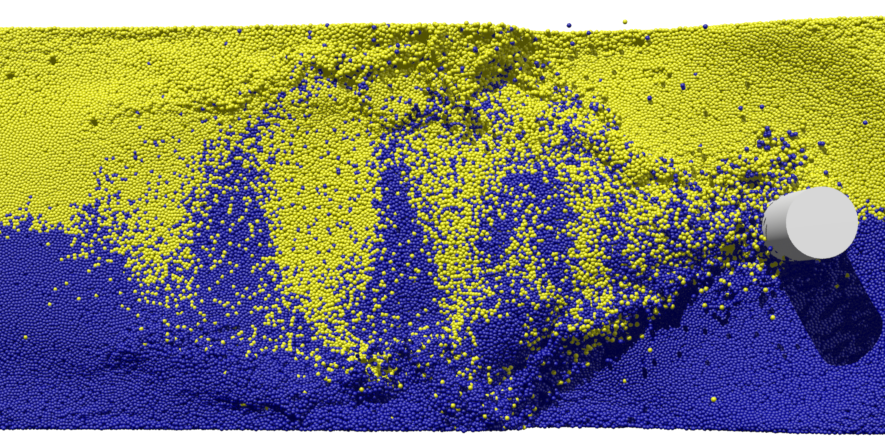
\includegraphics[width=0.31\textwidth]{figure/rod/fine210.png}
}
\subfigure{
\centering
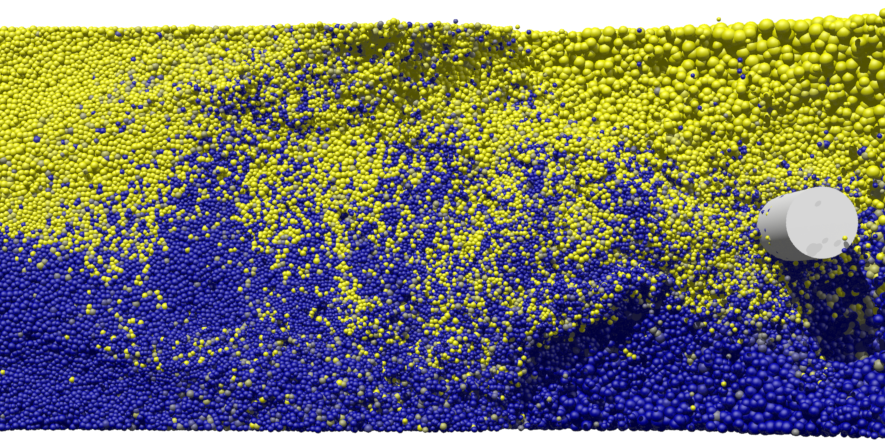
\includegraphics[width=0.31\textwidth]{figure/rod/mark215.png}
}
\subfigure{
\centering
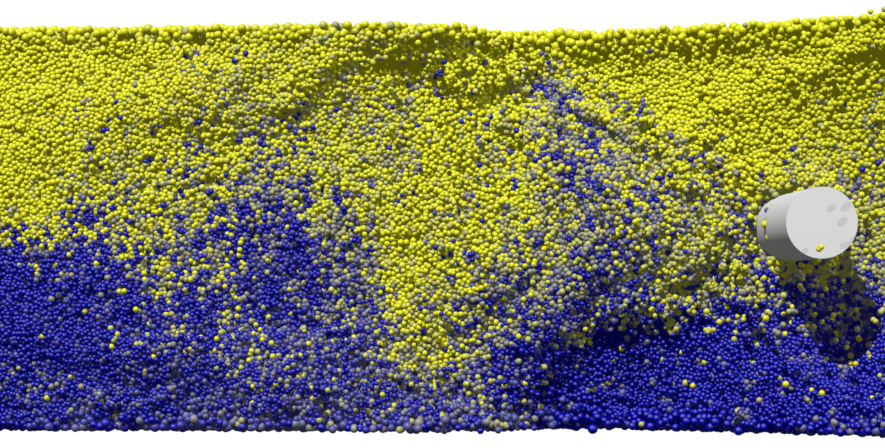
\includegraphics[width=0.31\textwidth]{figure/rod/surface215.png}
}

\setcounter{subfigure}{0}
\subfigure[High-resolution ($r=0.063\textrm{m}$).]{
\centering
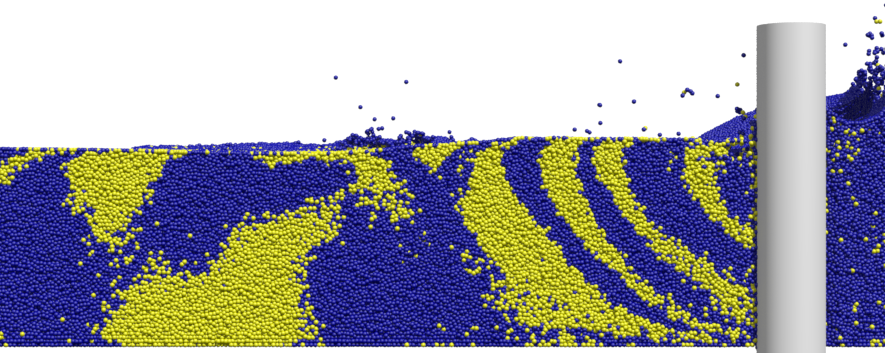
\includegraphics[width=0.31\textwidth]{figure/rod_side/fine210.png}
\label{fig:rod_fine}
}
\subfigure[Ours, $\tau^{max}_{cylinder} = 21$.]{
\centering
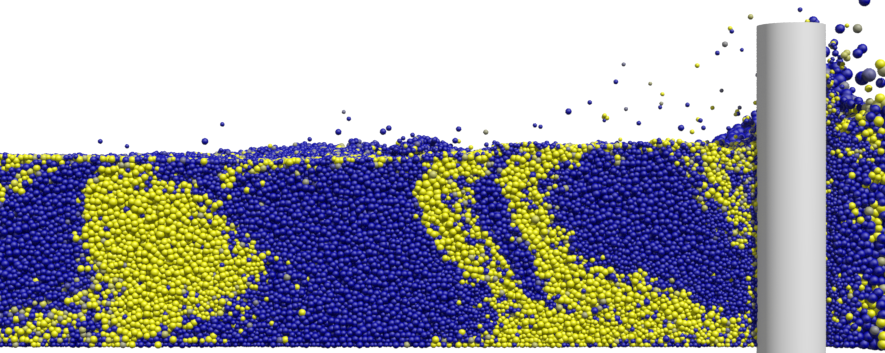
\includegraphics[width=0.31\textwidth]{figure/rod_side/mark215.png}
\label{fig:rod_mark}
}
\subfigure[Surface-based~\cite{Winchenbach17}.]{
\centering
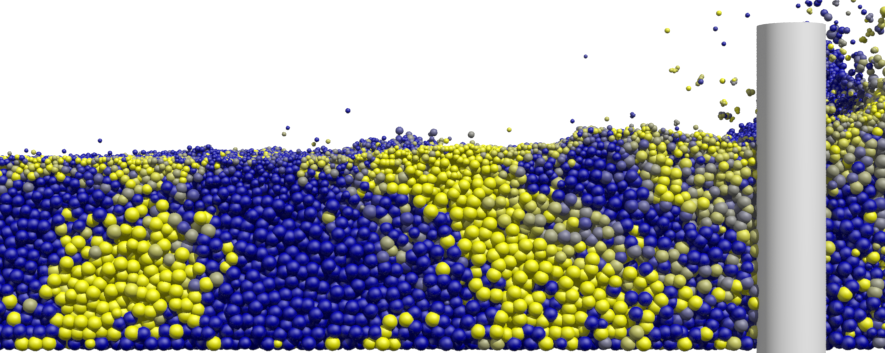
\includegraphics[width=0.31\textwidth]{figure/rod_side/surface215.png}
\label{fig:rod_surface}
}
\vspace{-0.7\baselineskip}
\caption{
Cylinder moving experiment, where the cylinder moves horizontally in the tank. The first row is the vertical view; the second row is a cross-section of the side view. Our method better reproduces the jagged (vertical view) and curved (side view) wave patterns in the high-resolution simulation. Adaptive methods use max particle size $r_{base} = 0.2$ and $\alpha = 32$.
}
\label{fig:rod}

\end{figure*}

A popular approach for boundary handling of SPH fluids is particle-based methods that represent the solid objects with particles \cite{Akinci12, Band18b}. However, for fluid simulation using adaptive methods, particle-based boundary representation may encounter the problem of size discrepancy between fluid and boundary particles. Another approach for boundary handling is the boundary integral method. Fujisawa et al.~\cite{Fujisawa15} used empirically derived functions to handle triangle-mesh boundaries. Koschier and Bender~\cite{Koschier17} precomputed the integral of boundary on a fixed grid, where the precomputing was rather expensive. Bender et al.~\cite{Bender19} improved this method by precalculating a volume term. Chang et al.~\cite{Chang20} integrated computer-aided design (CAD) mesh file boundary representation into SPH by converting the volume integral to surface integral. Winchenbach et al.~\cite{Winchenbach20} proposed a boundary integral method that supports adaptive SPH, which approximated the boundary integral locally at each particle with a plane based on the signed-distance field of the boundary object. Though the boundary handling for adaptive SPH has been well-studied, more attention needs to be paid to designing the adaptive mechanism dedicated to the fluid-solid boundary. So in this paper, we present a spatial adaptivity method with the boundary refinement mechanism for SPH fluid simulation to capture detailed interaction effects.

\section{Adaptive SPH}

\subsection{SPH Basics}

To simulate fluid behaviour, the SPH method~\cite{Koschier19} describes physical fluid motion according to the Navier-Stokes equation:
\begin{equation}
    \rho \frac{D\mathbf{v}}{Dt}=-\nabla p + \rho \upsilon \nabla^2 \mathbf{v} + \mathbf{f}_{ext},
\label{equ-2}
\end{equation}
where the change rate of the velocity $\mathbf{v}$ is determined by pressure $p$, density $\rho$, dynamic viscosity $\upsilon$ and external body force $\mathbf{f}_{ext}$.

To perform numerical computation, SPH discretizes the fluid into particles and calculates the physical attributes of each particle using the attributes from neighbouring particles and a kernel function $W$, as:
\begin{equation}
    A_i = \sum_j A_j \frac{m_j}{\rho_j} W(\mathbf{x}_i - \mathbf{x}_j, h_{ij}),
    \label{eq:sph_base}
\end{equation}
where $A$ is the physical attribute. $i$ is the current particle. $j$ denotes neighbouring particles of $i$, whose distance to $i$ is smaller than the support radius $h_{ij}$. $h_{ij} = (h_i + h_j) / 2$, where $h_i = 2r_i$ and $r$ is the particle diameter. $m$ is mass. $\mathbf{x}$ is position. This paper uses a cubic spline function for the kernel function $W$. Any value followed by the subscript $i$ or $j$ means the value of that particle.

According to Eqn.~\ref{eq:sph_base}, density located at particle $i$ can be approximated as:
\begin{equation}
    \rho_i = \sum_j m_j W_{ij},
    \label{eq:sph_density}
\end{equation}
where $W_{ij}$ is short for $W(\mathbf{x}_i - \mathbf{x}_j, h_{ij})$.

Using the state equation from Becker and Teschner~\cite{Becker07}, the pressure at the particle $i$ can be calculated as:
\begin{equation}
    p_i = B\left(\left(\frac{\rho_i}{\rho_0}\right)^\gamma - 1\right),
\end{equation}
where $B = \rho_0 c_s^2 / \gamma$. $\rho_0$ is the rest density denoting the density of the fluid without any compression. $c_s$ is the speed of sound in the fluid, which is often set to $100\textrm{m}/\textrm{s}$. $\gamma$ is set to $\gamma = 7$ for weakly compressible fluids.

The pressure force on the particle can then be computed as:
\begin{equation}
    \mathbf{F}_i^p = -m_i \sum_j m_j \left(
    \frac{p_i}{\rho_i^2} + \frac{p_j}{\rho_j^2}
    \right)\nabla W_{ij}.
\end{equation}

The viscosity force can be approximated as follows:
\begin{equation}
    \mathbf{F}_i^{vis} = 
    m_i \sum_j m_j \upsilon \left(\frac{\mathbf{v}_{ij}\cdot\mathbf{x}_{ij}}{|\mathbf{x}_{ij}|^2 + 0.01h_i^2}\right)\nabla W_{ij},
    % \left\{
    % \begin{array}{ll}
    %     m_i \sum_j m_j \upsilon \left(\frac{\mathbf{v}_{ij}\cdot\mathbf{x}_{ij}}{|\mathbf{x}_{ij}|^2 + 0.01h_i^2}\right)\nabla W_{ij} & \mathbf{v}_{ij}\cdot\mathbf{x}_{ij} < 0   \\
    %     \mathbf{0} & \mathbf{v}_{ij}\cdot\mathbf{x}_{ij} < 0 
    % \end{array}
    % \right.,
    \label{eq:vis}
\end{equation}
where $\mathbf{v}_{ij} = \mathbf{v}_i - \mathbf{v}_j$ is the relative velocity between $i$ and $j$. $\mathbf{x}_{ij} = \mathbf{x}_i - \mathbf{x}_j$.

The total force on a particle can be expressed as:
\begin{equation}
    \mathbf{F}_i = \mathbf{F}_i^p + \mathbf{F}_i^{adv} + \mathbf{F}_i^{bound},
\end{equation}
where $\mathbf{F}^{adv}$ is the advection force consisting of gravity $\mathbf{G}$, viscosity force $\mathbf{F}^{vis}$, and surface tension~\cite{Akinci13}. $\mathbf{F}^{bound}$ is the force from the boundary to the fluid, which is explained in Section \ref{sec:boundary}. The velocity and position of the particle are updated each time step with $\mathbf{v}_i := \mathbf{v}_i + \Delta t \mathbf{F}_i / m_i$, $\mathbf{x}_i := \mathbf{x}_i + \Delta t \mathbf{v}_i$, where $\Delta t$ is the length of the time step.

\subsection{Split-merge Based Adaptivity}

Winchenbach et al.~\cite{Winchenbach17} achieved SPH adaptivity by splitting and merging particles with strict conservation of the total fluid mass. In this method, the desired size for each particle is computed using a sizing function based on the distance to the fluid's free surface:
\begin{equation}
    m_i^{opt} = m^{base}\left(
    \frac{\mathrm{min}(|\phi_i^f|,|\phi_{max}|)}{|\phi_{max}|}
    (1 - \alpha) + \alpha
    \right),
    \label{eq:m_opt}
\end{equation}
where $m^{opt}$ is the optimal mass that is the desired mass for the particle. $\alpha$ is the adaptivity ratio that denotes the largest mass ratio allowed between particles. $m^{base}$ is the largest allowed particle mass. $\phi^f$ is the distance to the fluid's free surface similar to Horvath and Solenthaler \cite{Horvath13}, which is negative inside the fluid. $\phi_{max}$ is the max distance to the surface within which particles are refined. Eqn.~\ref{eq:m_opt} ensures that the optimal mass decreases linearly and smoothly as the distance to the free surface decreases.

\begin{figure}[b]
    \centering
    \subfigure[Splitting]{
        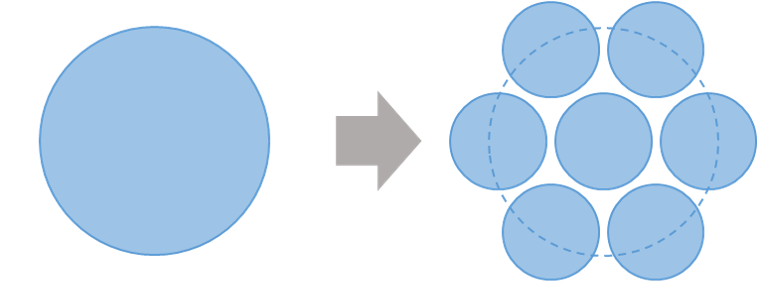
\includegraphics[width=0.29\columnwidth]{figure/split_schem/split.png}
    }
    \subfigure[Merging]{
        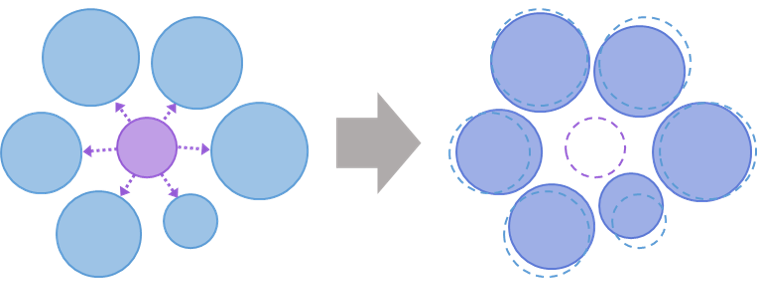
\includegraphics[width=0.29\columnwidth]{figure/split_schem/merge.png}
    }
    \subfigure[Redistribution]{
        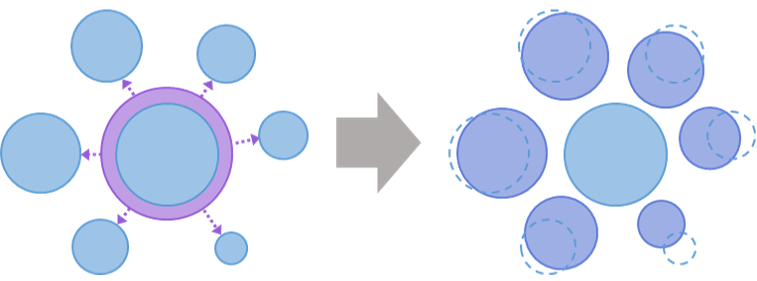
\includegraphics[width=0.29\columnwidth]{figure/split_schem/redistribute.png}
    }
    \vspace{-0.7\baselineskip}
    \caption{Schematic diagram of particle splitting, merging and redistribution.}
    \label{fig:split_schem}
\end{figure}

Splitting or merging is applied to each particle to adjust its mass towards $m^{opt}$ if necessary. To determine the operation each particle needs, the particles are classified into five categories according to the ratio between the particle's mass and the optimal mass, $m_i^{rel} = m_i / m_i^{opt}$. The five classes are $S$ ($m_i^{rel} < 0.5$), $s$ ($0.5 \leq m_i^{rel} \leq 0.9$), $o$ ($0.9 < m_i^{rel} < 1.1$), $l$ ($1.1 \leq m_i^{rel} \leq 2$), and $L$ ($2 < m_i^{rel}$)

Particles of class $L$ undergo splitting to become multiple smaller particles (Section \ref{sec:split}); particles of class $s$  are merged into nearby $s$ or $S$ particles by distributing all of its mass to nearby particles (Section \ref{sec:merge}); and particles of class $l$ redistribute their excess mass to nearby $s$ particles similarly to merging (Section \ref{sec:merge}). The process is shown schematically in Fig. \ref{fig:split_schem}.

\subsubsection{Splitting}
\label{sec:split}
Particles of class $L$ are split into $n$ children particles where $n = \lceil m_i / m_i^{opt} \rceil$. The mass and positions of children particles are determined using precomputed split patterns. They are further optimized online by solving a minimization problem on density error to reduce the error induced by splitting~\cite{Winchenbach21}. The other physical attributes of children particles are inherited from their parents.

\subsubsection{Merging and Redistribution}
\label{sec:merge}
Particles of class $s$ undergo merging, distributing all of their mass to nearby $s$ or $S$ particles, while particles of class $l$ redistribute their excess mass $m_i - m_i^{opt}$ to nearby $s$ particles. The distance between the mass-distributing particle $i$ and the mass-receiving particle $j$ must be within $h_i / 2$. The mass to distribute $m^{dist}$ is equally divided among the mass-receiving particles, while the other physical attributes are weight-averaged between $i$ and $j$ as:
\begin{equation}
    A_j^* = \frac{\frac{m^{dist}}{n}A_i + m_j A_j}{\frac{m^{dist}}{n} + m_j},
\end{equation}
where $A^*$ is the attribute's new value after redistribution, and $n$ is the number of mass-receiving particles.

\subsubsection{Techniques to Increase Stability}
Even with optimized splitting patterns and online optimization, splitting and merging can still introduce some density errors~\cite{Winchenbach21}. Temporal blending~\cite{Winchenbach17} and local viscosity~\cite{Winchenbach21} can increase the stability of particle splitting and merging.

Temporal blending is applied to particles that recently participated in splitting, merging, or mass redistribution. The original particle $o$ before splitting or redistributing mass is stored. Then, $o$ is used to modify the density and velocity of its children or particles that received mass from it. The blended density is computed as:
\begin{equation}
    \rho_i^{blended} = (1 - \beta) \rho_i + \beta \rho_o,
\end{equation}
where $\rho_o$ is the density of the original particle, computed using Eqn.~\ref{eq:sph_density}, but ignoring the density contribution from its children. $\beta$ is a temporal blending factor that is initialized to $0.5$ for particles generated in splitting and $0.2$ for particles involved in redistribution or merging.  Then, $\beta$ is decreased by $0.1$ every time step until it reaches $0$. $\rho_i^{blended}$ is used instead of $\rho_i$ in further computations.
The velocity of the original particle $\mathbf{v}_o$ is set to the average velocity of all its children particles and is used to update the original particle's position $\mathbf{x}_o$. The blended velocity $\mathbf{v}_i^{blended} = (1 - \beta) \mathbf{v}_i + \beta \mathbf{v}_o$ is used instead of $\mathbf{v}_i$ to update the particle's position $\mathbf{x}_i$.

In the local viscosity technique, the viscosity coefficient $\upsilon$ in Eqn.~\ref{eq:vis} is multiplied with a factor $1 + 0.5(\beta_i + \beta_j)/2$ to increase the viscosity of newly split, merged or redistributed particles locally, thus increasing stability.

\begin{figure*}
    \centering
    \subfigure[Ours, $\tau_{boat}^{max}=0$.]{
    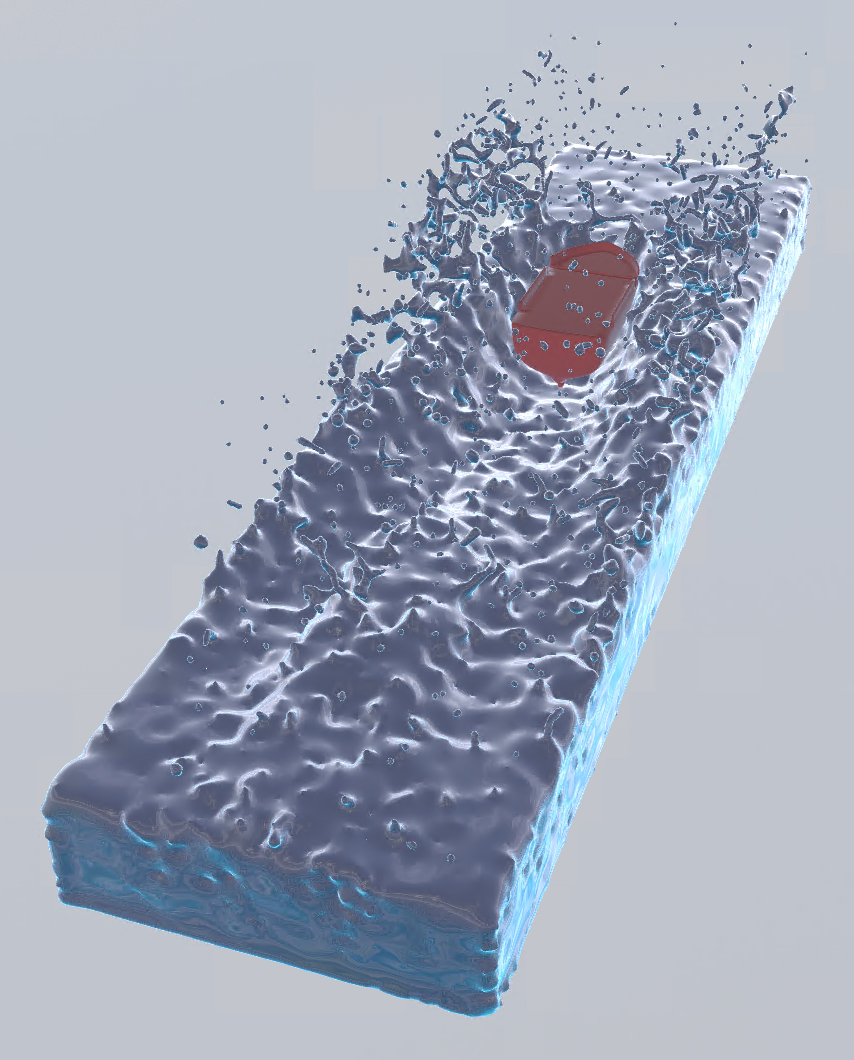
\includegraphics[width=0.18\textwidth]{figure/ship_reconstruct/bound.png}
    \label{fig:ship_our}
    }
    \subfigure[Ours, $\tau_{boat}^{max}=1$.]{
    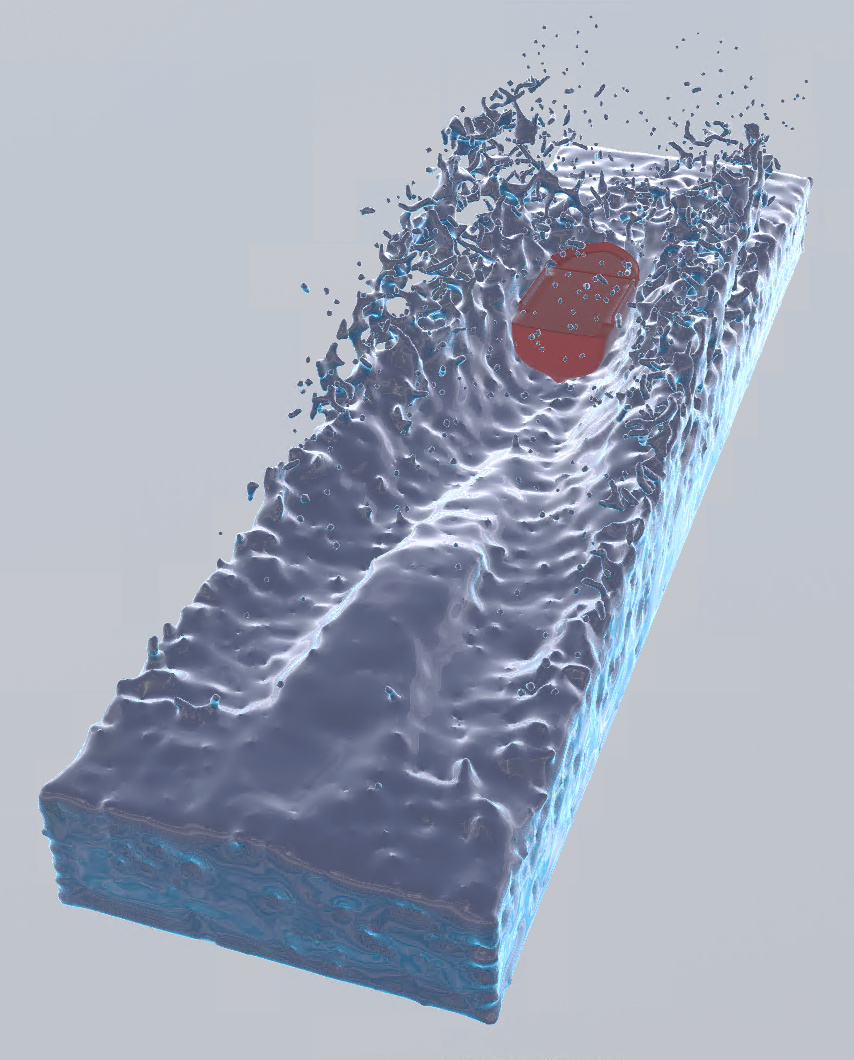
\includegraphics[width=0.18\textwidth]{figure/ship_reconstruct/mark.png}
    \label{fig:ship_mark}
    }
    \subfigure[Surface-based~\cite{Winchenbach17}.]{
    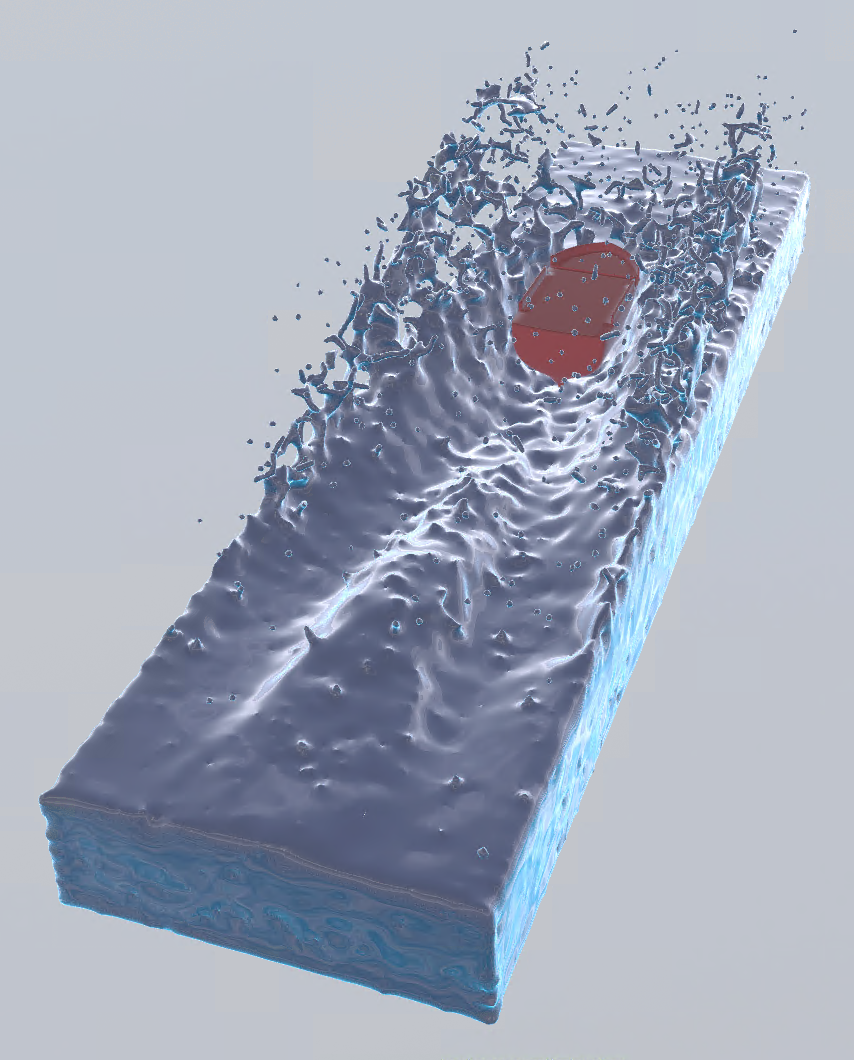
\includegraphics[width=0.18\textwidth]{figure/ship_reconstruct/surface.png}
    \label{fig:ship_w17}
    }
    \subfigure[Low-resolution.]{
    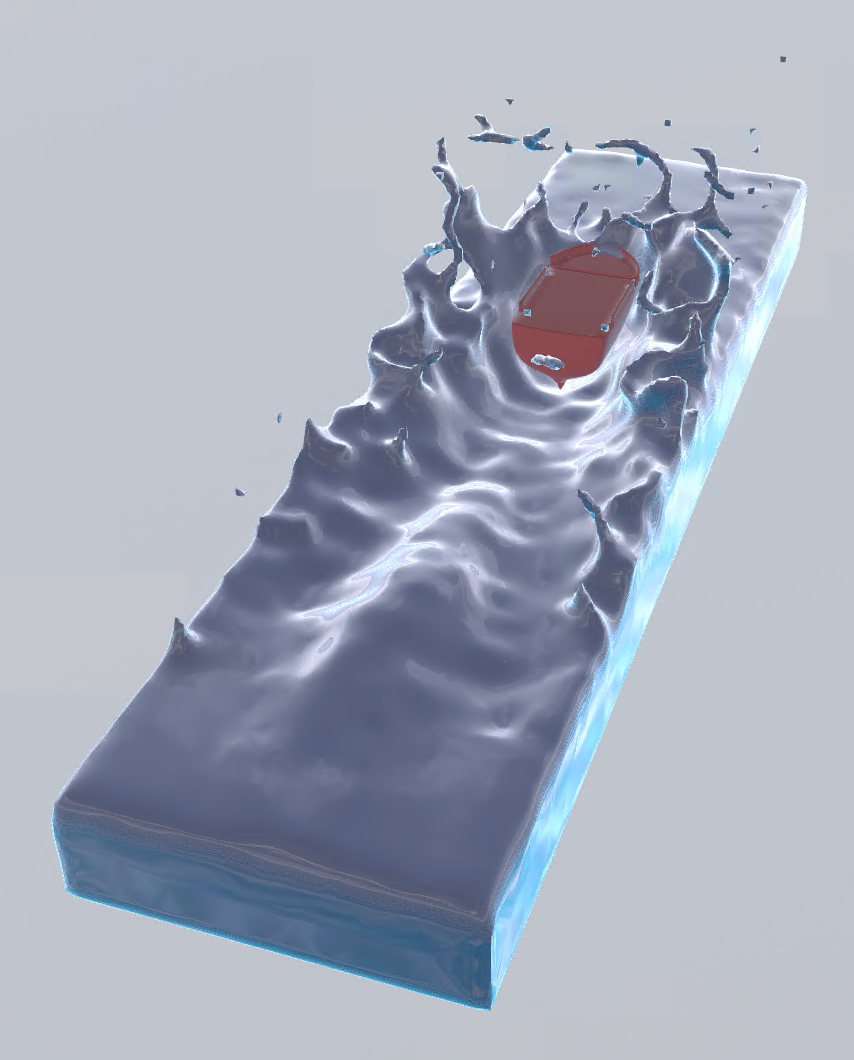
\includegraphics[width=0.18\textwidth]{figure/ship_reconstruct/coarse.png}
    \label{fig:ship_2}
    }
    \subfigure[High-resolution.]{
    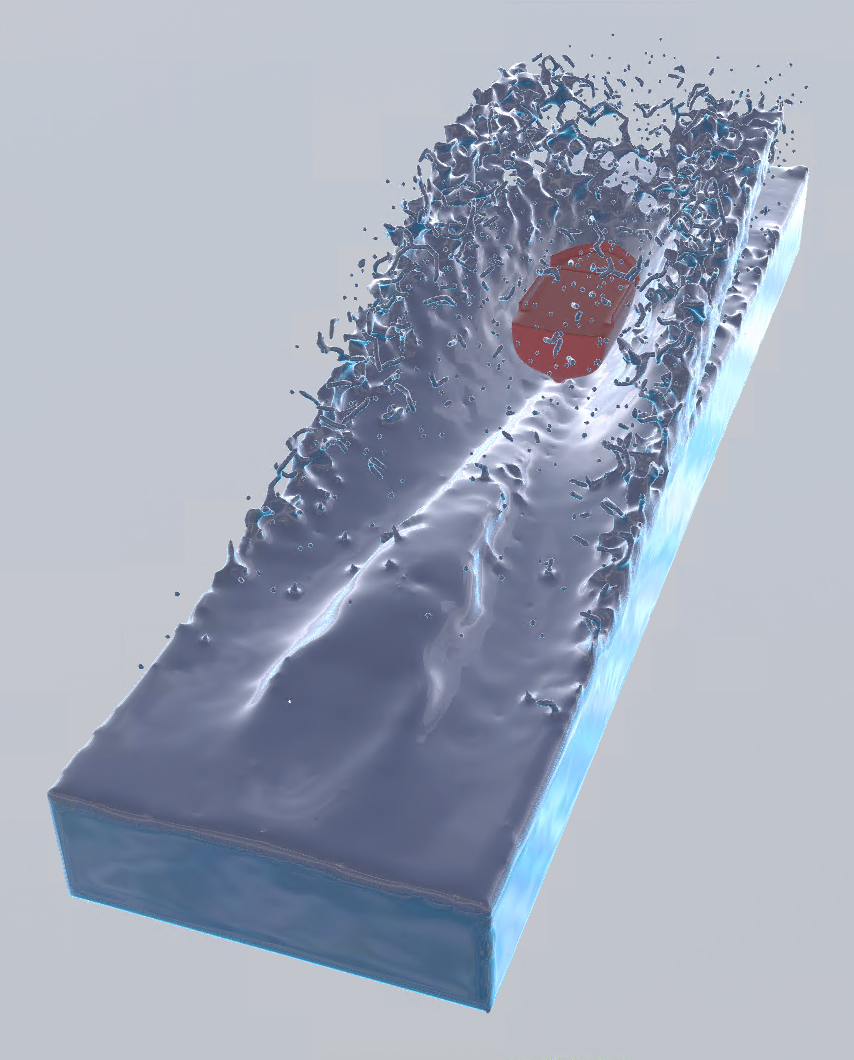
\includegraphics[width=0.18\textwidth]{figure/ship_reconstruct/fine.png}
    \label{fig:ship_063}
    }
    \caption{Surface reconstruction result of the boat-sailing experiment: (a), (b) and (c) are adaptive simulations using max particle size $r_{base} = 0.2$ and adaptive ratio $\alpha = 32$; (d) and (e) are uniform scale simulations with $r = 0.2$ and $r = 0.063$.}
    \label{fig:ship_reconstruct}
\end{figure*}


\section{Semi-analytic Boundary Handling}
\label{sec:boundary}

A suitable boundary handling method for adaptive SPH is proposed in \cite{Winchenbach20}. This method uses a local plane to approximate the boundary at each particle. The plane approximation is based on a discrete signed-distance field (SDF) evaluated before simulation. The plane's distance $d$ to the particle equals the SDF magnitude at the particle's position, and the normal vector of the plane is the normalised SDF gradient. To approximate the boundary's contribution, the integral of the kernel function $W$ is evaluated over the region on the side of the plane that contains the boundary:
% \begin{equation}
%     \lambda'(d) = \left\{
%     \begin{array}{ll}
%         \vspace{5pt}
%         \makecell[l]{\frac{1}{30}[81q^6 - 144q^5+ \\ 80q^3 -42q + 15]} & 0 \leq q \leq 0.5\\
%         \vspace{5pt}
%         \makecell[l]{\frac{-8}{15}[2q^6 - 9q^5 + 15q^4 \\ - 10q^3 + 3q - 1]} & 0.5 < q \leq 1 \\
%         \makecell[l]{1-\lambda'(-q)} & -1 \leq q < 0 
%     \end{array}
%     \right.,
% \end{equation}
\begin{equation}
    \lambda'(d) = \left\{
    \begin{array}{ll}
        \vspace{5pt}
        \makecell[l]{\frac{1}{30}[81q^6 - 144q^5+ 80q^3 -42q + 15]} & \hspace{2em} 0 \leq q \leq 0.5\\
        \vspace{5pt}
        \makecell[l]{\frac{-8}{15}[2q^6 - 9q^5 + 15q^4 - 10q^3 + 3q - 1]} & \hspace{2em} 0.5 < q \leq 1 \\
        \makecell[l]{1-\lambda'(-q)} & \hspace{2em} -1 \leq q < 0 
    \end{array}
    \right.,
\end{equation}
where $q = d / h_i$.

A penalty term is introduced to penalize solid penetration: $\beta(d) = 1 - d / h_i$. The penalty term is directly multiplied onto $\lambda'(d)$, obtaining the corrected value $\lambda(d) = \beta(d) \lambda'(d)$.

% $\partial\beta(d) / \partial(d) = - 1 / h_i$
% $\nabla\lambda'(d) = \partial\beta / \partial(d) \mathbf{n} \lambda'(d) + \beta(d)\nabla'(d)$.

The density equation Eqn.~\ref{eq:sph_density} is then modified to consider the boundary:
\begin{equation}
    \rho_i = \sum_j m_j W_{ij} + \sum_b \rho_0 \lambda_i^b,
\end{equation}
where $b$ denotes the boundary object(s). $\lambda_i^b = \lambda(\mathrm{sdf}^b(\mathbf{x}_i))$, where $\mathrm{sdf}^b(\mathbf{x}_i)$ is the signed-distance to $b$ from the position of $i$.

The pressure at the boundary can be mirrored~\cite{Akinci12} or extrapolated~\cite{Band18b} from the pressure of nearby fluid particles. In the case of pressure mirroring, the pressure force from the boundary is:
\begin{equation}
    \mathbf{F}_{i \leftarrow b}^p = -m_i \rho_0 \frac{p_i}{\rho_i^2} \nabla\lambda_i^b.
    \label{eq:bound_p}
\end{equation}
The friction between the fluid and solid follows the Coulomb model, which is proportional to the boundary's pressure force on the particle:
\begin{equation}
    \mathbf{F}_{i\leftarrow b}^{fric} = \mu ||\mathbf{F}_{i\leftarrow b}^p|| \mathbf{t}_{ib},
    \label{eq:bound_fric}
\end{equation}
where $\mathbf{t}_{ib}$ is a unit vector pointing to the direction of relative tangential velocity between fluid and boundary.

The total force from the boundary objects to a particle is $\mathbf{F}_i^{bound} = \sum_b (\mathbf{F}_{i \leftarrow b}^p + \mathbf{F}_{i\leftarrow b}^{fric})$.

\vspace{-0.5\baselineskip}

\begin{algorithm}[htb]
\par\setlength\parindent{2em}
\noindent \textbf{SPH Computation} 

Establish neighbour list

Compute and blend density

Calculate advection forces

Compute fluid pressure

Apply boundary pressure and friction

Update and blend velocity

Update position

\noindent \textbf{Adaptive Mechanism} 

\textcolor[RGB]{71,156,233}{Compute $\phi^b$ from boundary SDF (Eqn.~\ref{eq:bound_distance})}

\textcolor[RGB]{71,156,233}{Wake flow preservation (Algorithm \ref{alg:two})}

\textbf{if} combine surface-based: Detect surface

\textcolor[RGB]{71,156,233}{Calculate optimal mass (Eqn.~\ref{eq:refine_bound})}

Splitting, merging and redistribution

\caption{Boundary refinement for SPH. New steps in our method are marked blue.}
\label{alg:one}
\end{algorithm}

\section{Adaptive Boundary Coupling}
\label{sec:adaptive_our}

The region near the boundary objects is often of interest in fluid-boundary coupling. Therefore it is desirable to use the refined particles near the important boundary objects to emphasise the details of boundary coupling. However, refining the entire surface can cause an unnecessary increase in particle number. Previous work~\cite{Winchenbach17} refines particles only near the free surface of the fluid, which cannot cover the entire boundary region and can cause detail loss in boundary coupling. Moreover, in some cases, only the region near the boundary object is of interest, such as a ship sailing on a vast water surface.

Given the above problems, we propose a boundary refinement method to refine particles near specific boundary objects. The method can either be used alone to refine only near the boundary or combined with surface-based refinement schemes~\cite{Winchenbach17} to refine both the surface and the boundary regions, which is outlined in Algorithm \ref{alg:one}.

To achieve particle refinement near boundary objects, we modify the sizing function of Eqn.~\ref{eq:m_opt} to consider the distance to boundary objects. Instead of optimizing particle mass according to the distance to the free surface $\phi^f$, we use the distance to boundary objects to define a value $\phi^b$ to adjust the particle size:
\begin{equation}
    \phi_i^b = \min\left(\max_{b^*}\left(-\mathrm{sdf}^{b^*}(\mathbf{x}_i) + \phi_{b^*}^{fine}\right), 0\right),
    \label{eq:bound_distance}
\end{equation}
where $b^*$ denotes the interested boundary objects near which the fluid particles should be refined. $\phi_{b^*}^{fine}$ is a user-controlled parameter: all particles with distance to $b^*$ smaller than $\phi_{b^*}^{fine}$ are refined to the smallest scale. We use $\phi_{b^*}^{fine} = h_i$ unless explicitly mentioned.

To only refine the region near the boundary, one can replace $\phi_i^f$ with $\phi_i^b$ in Eqn.~\ref{eq:m_opt}, namely:
\begin{equation}
    m_i^{opt} = m^{base}\left(
    \frac{\mathrm{min}(|\phi_i^b|,|\phi_{max}|)}{|\phi_{max}|}
    (1 - \alpha) + \alpha
    \right),
    \label{eq:refine_bound}
\end{equation}
and to refine both near the boundary region and the fluid surface, one should substitute $\phi_i^f$ in Eqn.~\ref{eq:m_opt} with $\phi_i = \max(\phi_i^b, \phi_i^f)$.

\begin{figure*}[htpb]
    \centering
    \subfigure[Ours, $\tau_{boat}^{max} = 0$.] { 
        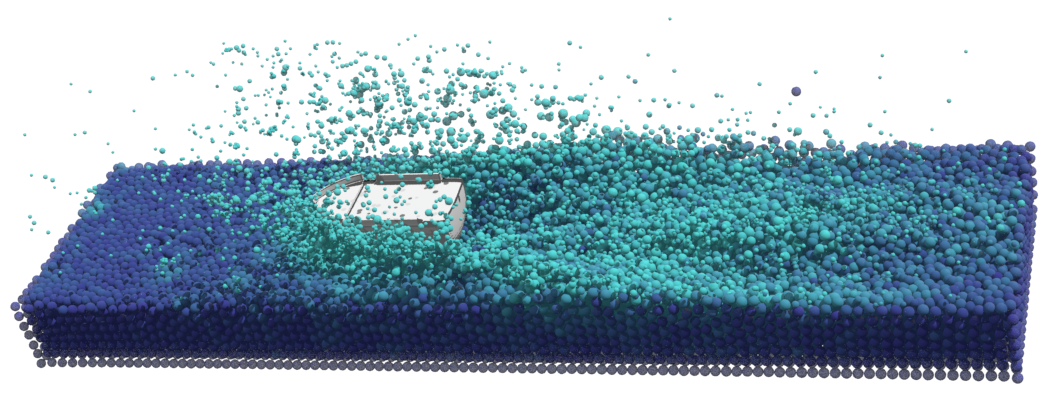
\includegraphics[width=0.31\textwidth]{figure/ship/bound90.png} 
    } 
    \subfigure[Ours, $\tau_{boat}^{max} = 1$.] {  
        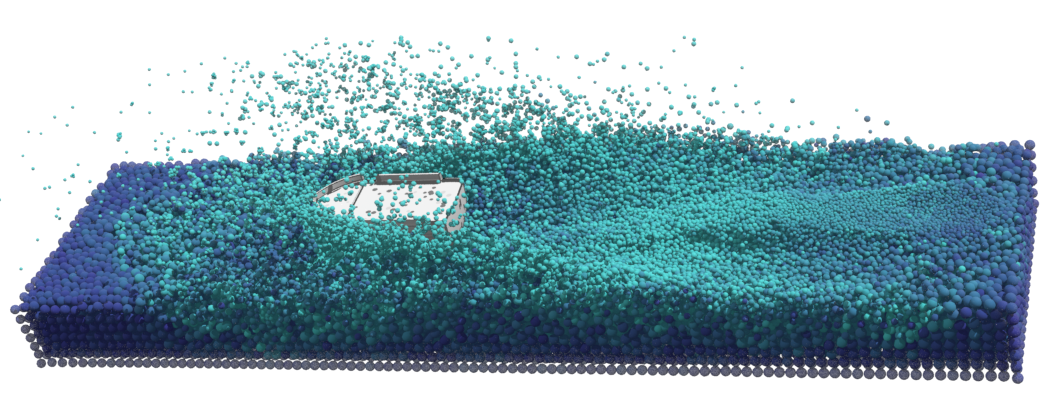
\includegraphics[width=0.31\textwidth]{figure/ship/mark90.png} 
    } 
    \subfigure[Surface-based~\cite{Winchenbach17}.] {  
        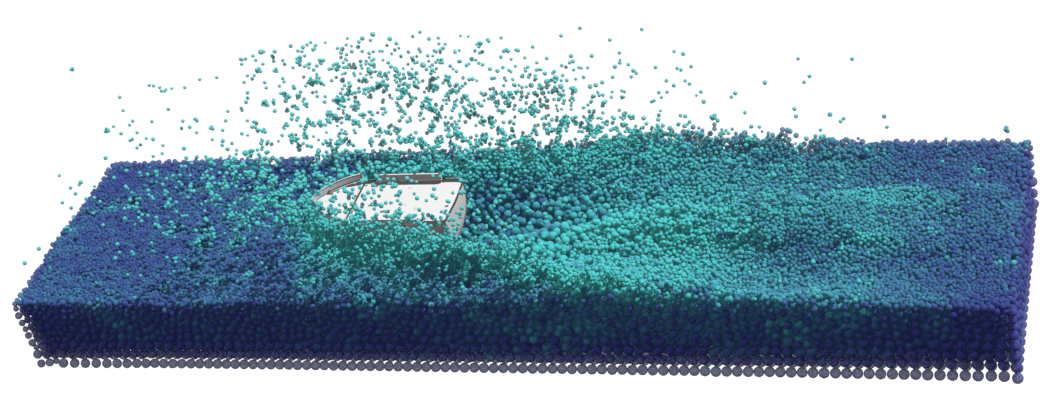
\includegraphics[width=0.31\textwidth]{figure/ship/surface90.png} 
    } 
    \subfigure[Low-resolution ($r = 0.2\mathrm{m}$).] { 
        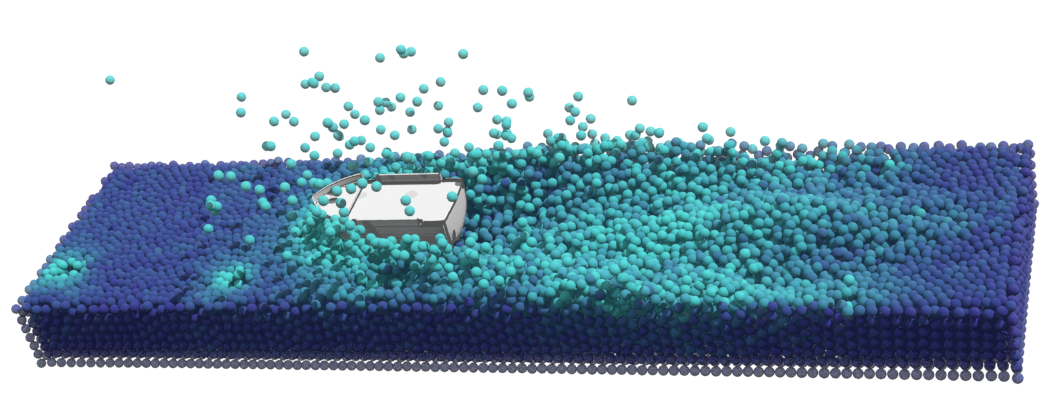
\includegraphics[width=0.31\textwidth]{figure/ship/coarse90.png} 
    } 
    \subfigure[High-resolution ($r = 0.063\mathrm{m}$).] { 
        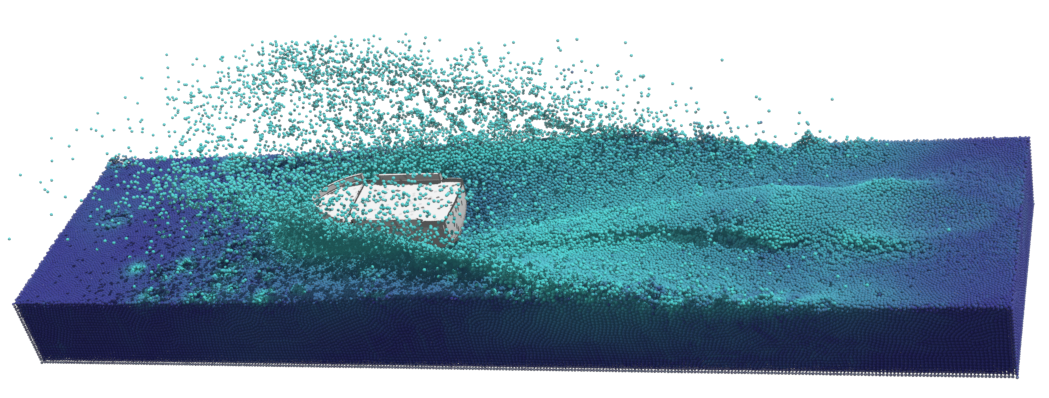
\includegraphics[width=0.31\textwidth]{figure/ship/fine90.png} 
    } 
    \vspace{-0.7\baselineskip}
    \caption{Boat-sailing experiment. Adaptive methods use $r_{base} = 0.2$ and $\alpha = 32$.}
    \label{fig:ship}
\end{figure*}

\subsection{Wake Flow Preservation by Delaying Merge}
\label{sec:wake_flow}

For scenarios where the fluid flows past the boundary object or the boundary object moves through the fluid, interesting wake flow effects are generated behind the boundary object, such as the wave behind a ship moving through water. However, when using $\phi_i^b$ to determine particle size, the wake flow loses detail because the optimal mass quickly returns to the largest value as the boundary object moves away from the particle. Consequently, the particles in the wake flow merge into larger particles, reducing the detail level.

To preserve wake flow detail, we inhibit the particle merging process if the particle was recently in the vicinity of the boundary, as Algorithm \ref{alg:two} shows. For each interested boundary object $b^*$, the user can set a duration to delay merging $\tau^{max}_{b^*}$ for particles that have flowed around it, and each particle tracks its remaining duration to delay merging, denoted as $\tau_i$. Every time step, for each particle $i$ and each interested boundary object $b^*$, if the particle satisfies $\mathrm{sdf}^{b^*}(\mathbf{x}_i)\leq h_i$ , we set its remaining duration $\tau_i := \tau^{max}_{b^*}$ if the duration is not already longer. The duration is decremented at each time step by the time step length $\Delta t$ as $\tau_i:=\tau_i-\Delta t$. As long as the particle satisfies $\tau_i > 0$, $\phi^b_i$ is not allowed to decrease: if the newly computed value $\phi^{b}_{i,t}$ for the time step $t$ is lower than the previous value $\phi^{b}_{i,t-1}$, we set it to $\phi^{b}_{i,t} := \phi^{b}_{i,t-1}$. To retain the smoothness of the $\phi^b$ field, the $\phi^b_i$ values for $\tau_i > 0$ are then propagated to surrounding particles using the method from Horvath and Solenthaler \cite{Horvath13}. This approach effectively delays particle merging in the wake flow by the time length of $\tau^{max}_{b^*}$.

\vspace{-0.5\baselineskip}

\begin{algorithm}[htb]
\par\setlength\parindent{2em}
\noindent \textbf{for each} particle $i$ 

\textbf{for each} interested boundary object $b^*$:

\hspace{2em}\textbf{if} $\mathrm{sdf}^{b^*}(\mathbf{x}_i)\leq h_i$:

\hspace{2em}\hspace{2em}set duration $\tau_i:=\mathrm{max}(\tau_{b^*}^{max},\tau_i)$
    
decrement duration $\tau_i:=\tau_i-\Delta t$
    
\textbf{if} $\tau_i>0$:
    
\hspace{2em}$\phi_{i,t}^b:=\mathrm{max}(\phi_{i,t}^b,\phi_{i,t-1}^b)$

\caption{Wake flow preservation.}
\label{alg:two}
\end{algorithm}

\vspace{-1.5\baselineskip}

\section{Results and Discussions}

To test the effectiveness and capabilities of our method, in this section, we use multiple scenarios to compare the proposed approach with simulations of uniform particle scale and the surface-based state-of-the-art SPH adaptive scheme~\cite{Winchenbach17}, which adapts resolution near the free surface.

We use Weakly Compressible SPH~\cite{Becker07} for fluid simulation and the semi-analytic boundary handling method proposed in~\cite{Winchenbach20} for boundary coupling. The time step length is determined using the CFL condition with a scaling parameter of $0.5$. Surface reconstruction and rendering are conducted using Houdini and mantra with Intel Xeon Gold 5218. All simulations are coded using the Taichi programming language~\cite{hu2019taichi} and run on an NVIDIA Tesla V100 GPU.

\subsection{Efficiency Comparison}

Efficiency is a crucial aspect of adaptive simulation mechanisms. We show that our method can produce a similarly detailed result using fewer particles than the surface-based adaptive mechanism~\cite{Winchenbach17} and is more vivid than a low-resolution simulation. 


\paragraph{Boat-sailing}

In this scenario, a boat sails quickly across a calm fluid surface, stirring up waves and splashes around and behind the body. For the adaptive methods, we use the max particle size $r_{base} = 0.2$ and an adaptive ratio $\alpha = 32$ and choose $\phi_{b^*}^{fine} = 0$ in our method. For uniform size simulations, we perform a low-resolution and a high-resolution simulation using $r = 0.2$ and $r = 0.063$, where the particle size respectively equals the largest and smallest particle size in adaptive simulation. The particles are colour-coded according to velocity.

Fig.\ref{fig:ship_reconstruct} and Fig.\ref{fig:ship} show the experimental results rendered with reconstructed fluid surface and particles, respectively. Considering the splashes around the ship, the visual level of detail is similar between the previous surface-based method~\cite{Winchenbach17} (Fig.\ref{fig:ship_w17}) and our method with or without wake flow preservation (Fig.\ref{fig:ship_mark}, \ref{fig:ship_our}). The three adaptive results are all much more detailed than the uniform low-resolution simulation (Fig.\ref{fig:ship_2}), though they may lack some detail compared to high-resolution (Fig.\ref{fig:ship_063}). For the wake flow effect, the result of our method without wake flow preservation (Fig.\ref{fig:ship_our}) is relatively coarse, but when wake flow preservation is added to our method (Fig.\ref{fig:ship_mark}), the visual detail level is comparable to the surface-based method (Fig.\ref{fig:ship_w17}).

To evaluate the efficiency of the proposed method, the particle count and time consumption using different methods are plotted in Fig.\ref{fig:ship_data}. The solid lines show the particle count, and the dashed lines show the time consumption. It can be seen that the uniform low-resolution simulation uses the least particles. While our adaptive method with $\tau_{boat}^{max} = 0$ increases the particle count slightly. Further, our method with $\tau_{boat}^{max} = 1$ begins with a low particle count, which increases since frame $65$ when the boat starts moving and producing wake flow, and decreases back to a low value after frame $107$ when the boat leaves the simulated zone because the duration to delay merging for the wake flow has expired. Under both conditions, our method significantly reduces the average particle count over time compared to the surface-based method~\cite{Winchenbach17} and the high-resolution simulation. The time consumption curves follow a similar trend. This experiment shows that our method can reduce the time cost compared to the state-of-the-art surface-based adaptive mechanism~\cite{Winchenbach17} with no or negligible negative influence on visual quality.

\begin{figure*}
    \centering
    \subfigure[Boat-sailing experiment.]{
    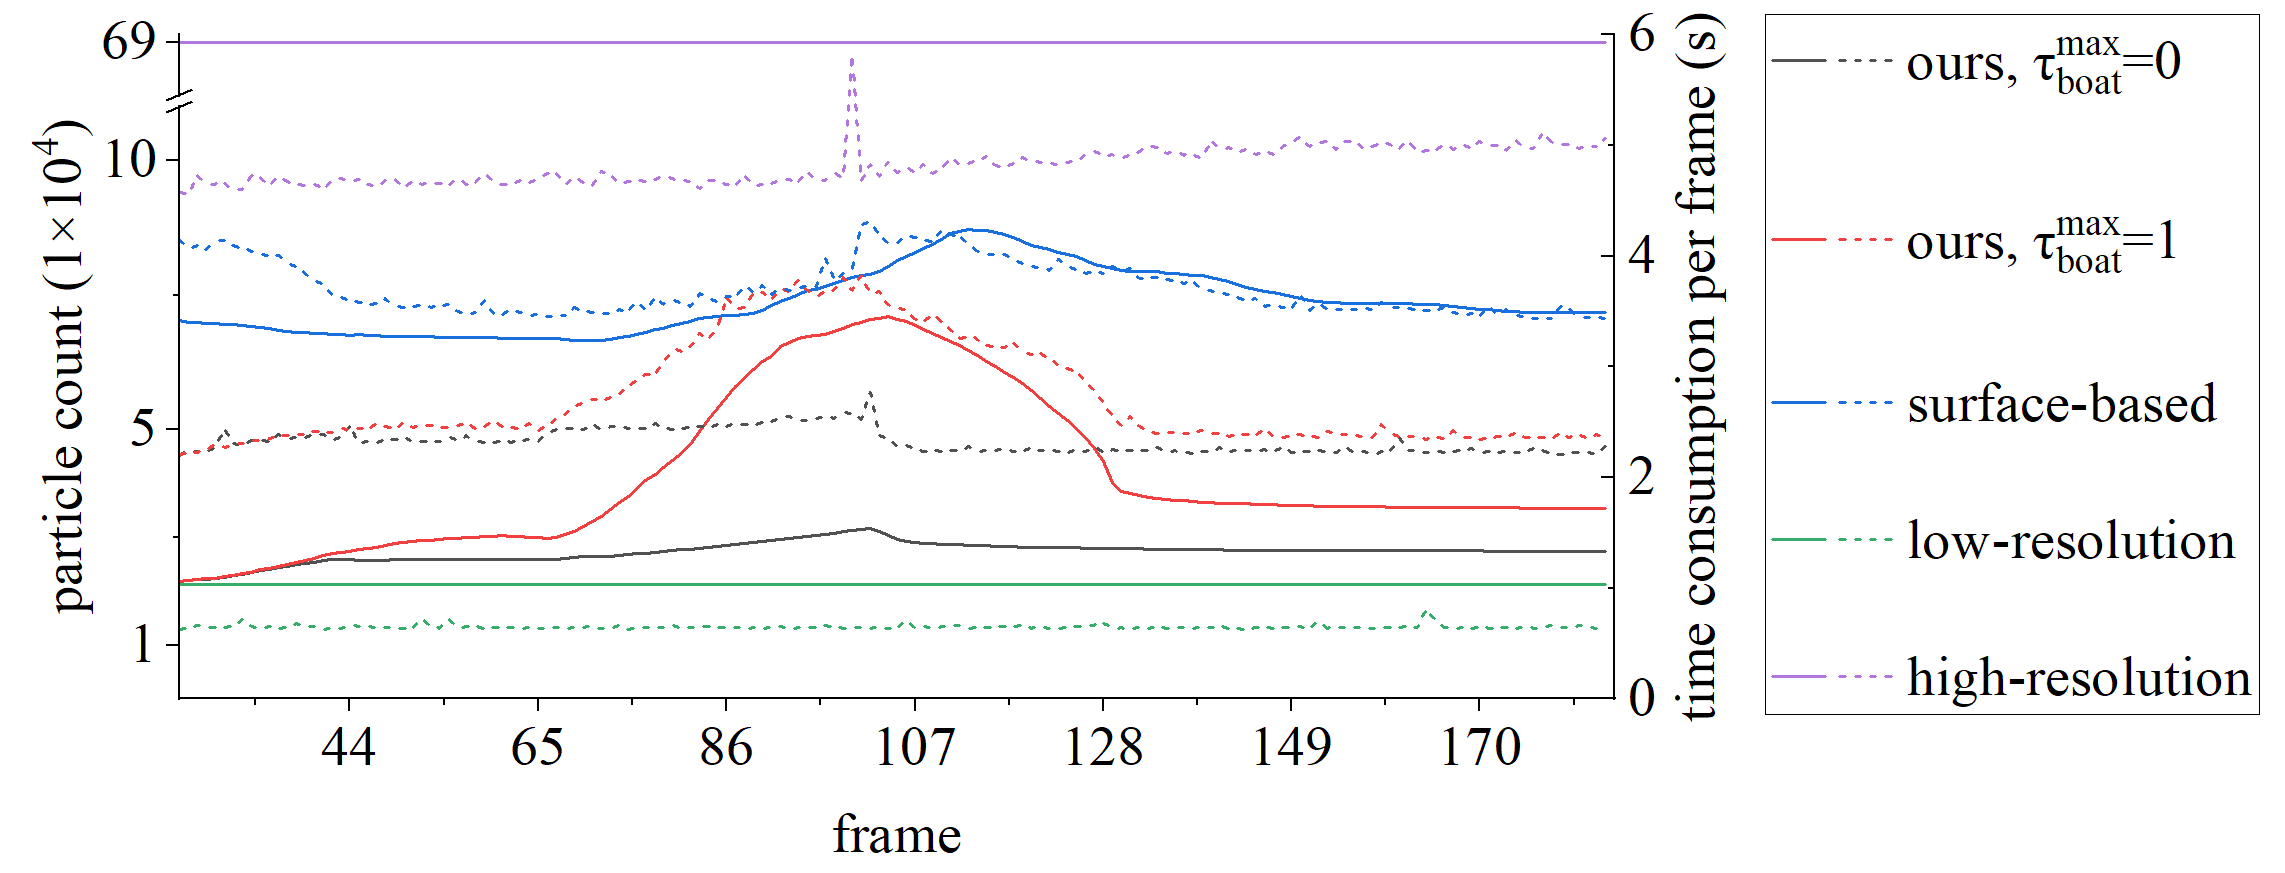
\includegraphics[width=0.635\textwidth]{figure/data/ship.png}
    \label{fig:ship_data}
    }
    \subfigure[Cylinder moving experiment.]{
    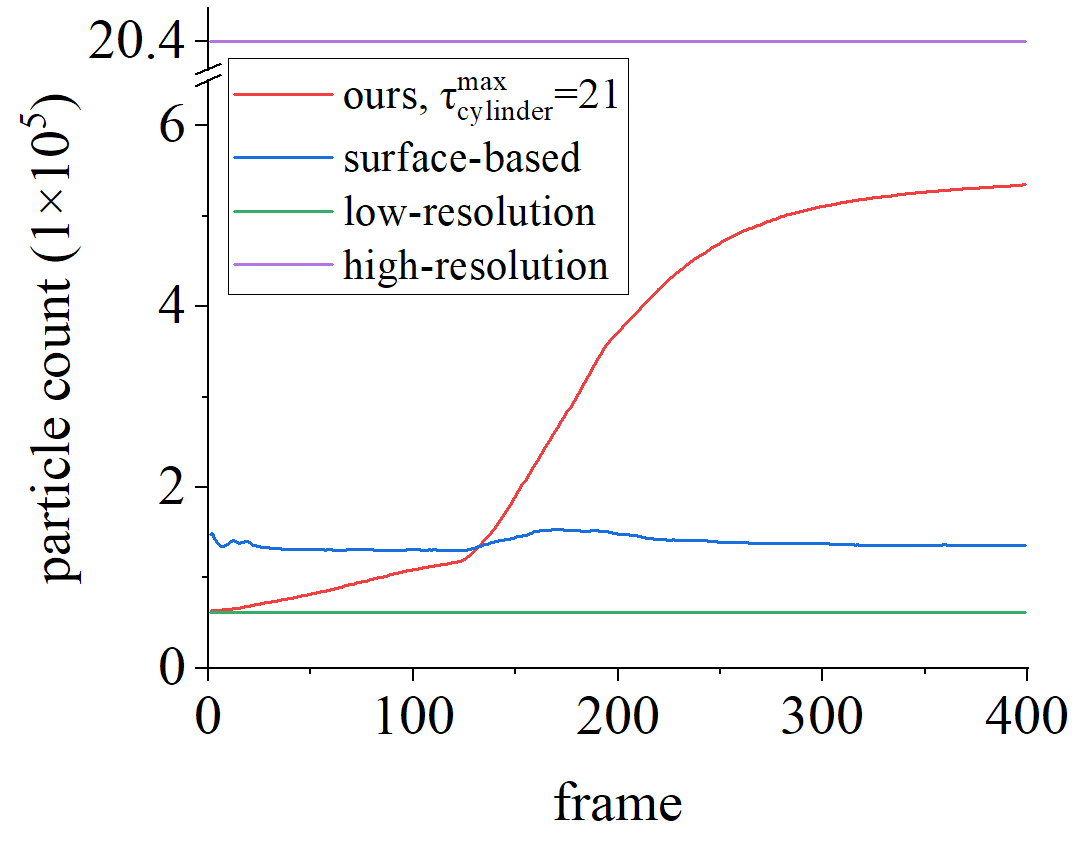
\includegraphics[width=0.3\textwidth]{figure/data/rod_count.png}
    \label{fig:rod_count}
    }
    \vspace{-0.7\baselineskip}
    \caption{Particle count and time consumption in boat-sailing and cylinder moving experiment. Solid lines denote particle count; dashed lines denote time consumption. One frame equals $1/24\mathrm{s}$.}
    
\end{figure*}

\subsection{Effect Evaluation}


\paragraph{Cylinder moving}

Fig.\ref{fig:rod} shows an experiment where a cylinder is moved horizontally through a water tank in a straight line to generate a wave pattern. The particles are coloured according to whether their initial positions are on one side of the moving path of the cylinder. A jagged pattern can be seen from the vertical view (first row), and curved patterns can be seen from the side view of a cross-section (second row). Fig.\ref{fig:rod_fine} shows the result of a uniformly scaled high-resolution simulation performed using the smallest allowed particle size in the two adaptive simulations, $r = 0.063$, which should be the most accurate among the three simulations. Fig.\ref{fig:rod_mark} uses our boundary refinement method where particles are adaptively refined near the cylinder. We use $\tau_{cylinder}^{max} = 21$, which is longer than the simulation duration, to prevent wake flow merging for the entire simulation to achieve a high level of detail. Fig.\ref{fig:rod_surface} uses surface-based refinement~\cite{Winchenbach17}. The two adaptive simulations use $r_{base} = 0.2$ and $\alpha = 32$. Compared to the surface-based method, our method is more similar to the high-resolution simulation in terms of the size and number of jags from the vertical view and the shape of the curved pattern in the cross-section, indicating our method can achieve a better accuracy compared to surface-based method~\cite{Winchenbach17} under certain settings.

The particle count of the cylinder moving experiment is displayed in Fig.\ref{fig:rod_count}. Our method uses a larger number of particles compared to the surface-based method~\cite{Winchenbach17} to achieve higher accuracy, but the particle count is still considerably lower than the high-resolution simulation.

\paragraph{Propeller spinning}

In this experiment, a propeller is fully submerged in the fluid and spins horizontally to generate turbulence. We use this scenario to demonstrate the ability of our method to be combined with surface-based refinement~\cite{Winchenbach17}.

Fig.\ref{fig:prop} shows the particle view of a cross-section of the propeller spinning experiment. From Fig.\ref{fig:prop_union}, it can be seen that the particle size is refined both near the surface and around the propeller. Compared with only using surface-based refinement as in Fig.\ref{fig:prop_surface}, the combined method can generate more details in a vortex, as shown in the zoomed-in areas, and also has a more similar shape to the vortex in a high-resolution simulation (Fig.\ref{fig:prop_fine}). This experiment shows that adding our method to the surface-based method~\cite{Winchenbach17} can enhance dynamic details produced by boundary coupling.

\begin{figure}[htbp]

\centering
\subfigure[High-resolution ($r=0.063\textrm{m}$).]{
\centering
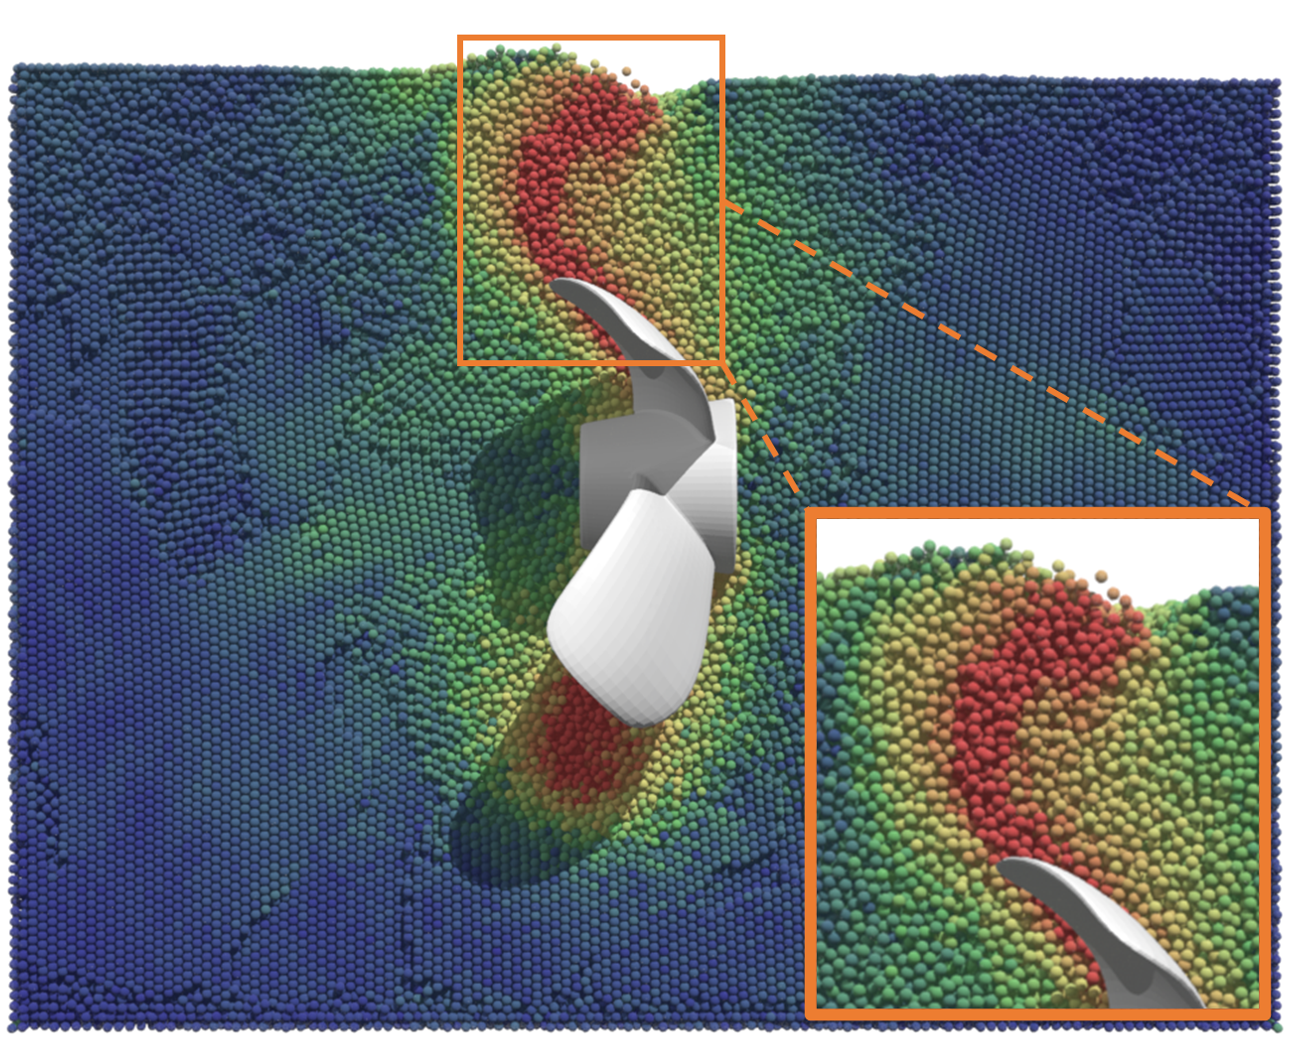
\includegraphics[width=0.31\textwidth]{figure/prop/fine.png}
\label{fig:prop_fine}
}
\subfigure[Ours + surface-based~\cite{Winchenbach17}.]{
\centering
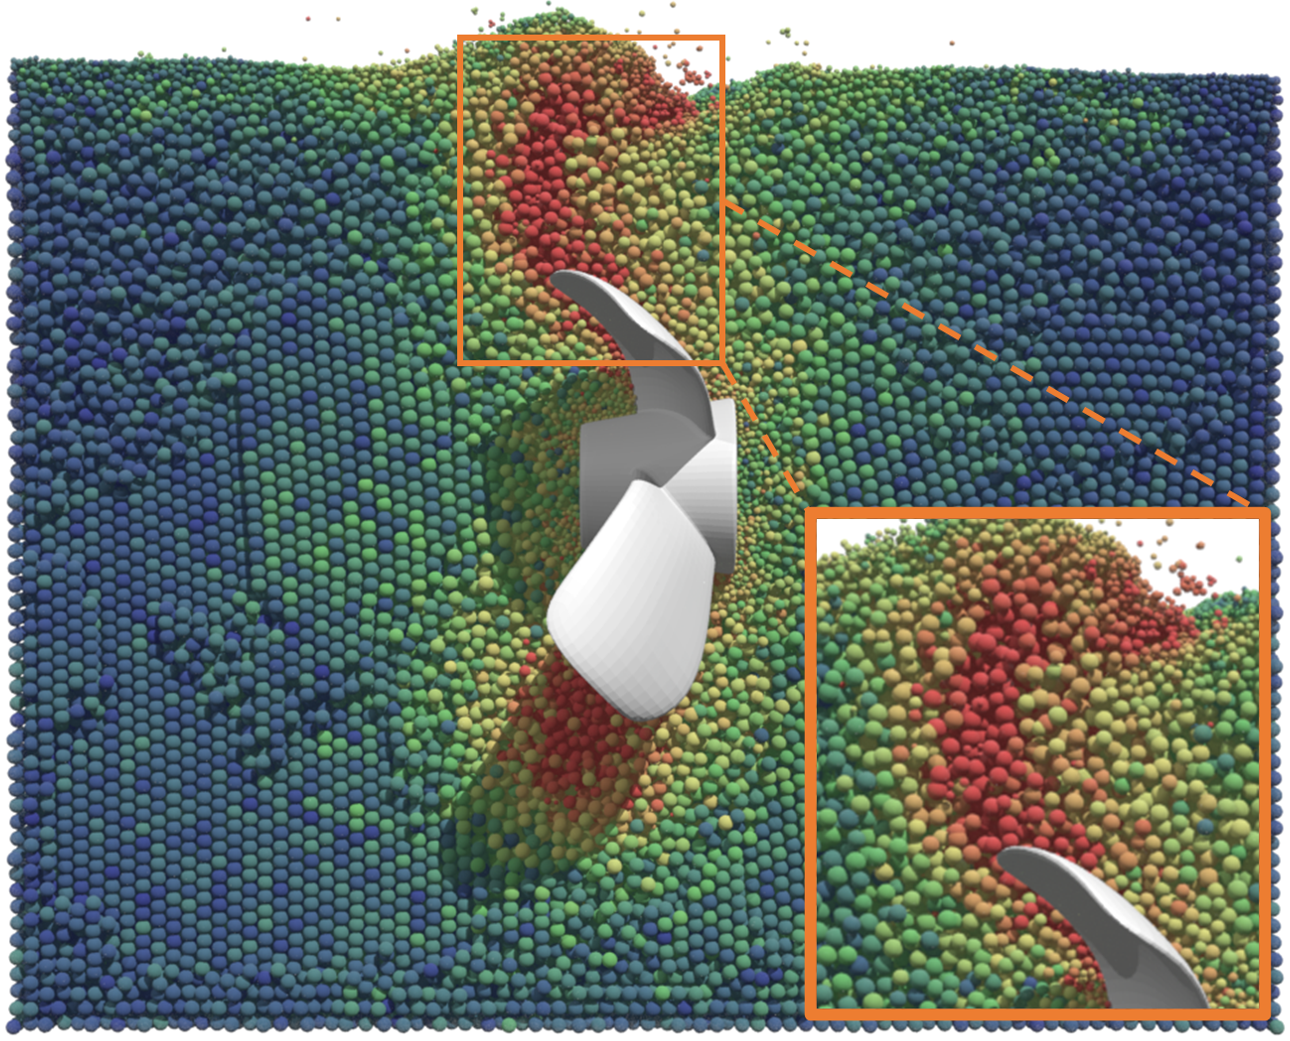
\includegraphics[width=0.31\textwidth]{figure/prop/union.png}
\label{fig:prop_union}
}
\subfigure[Only surface-based.]{
\centering
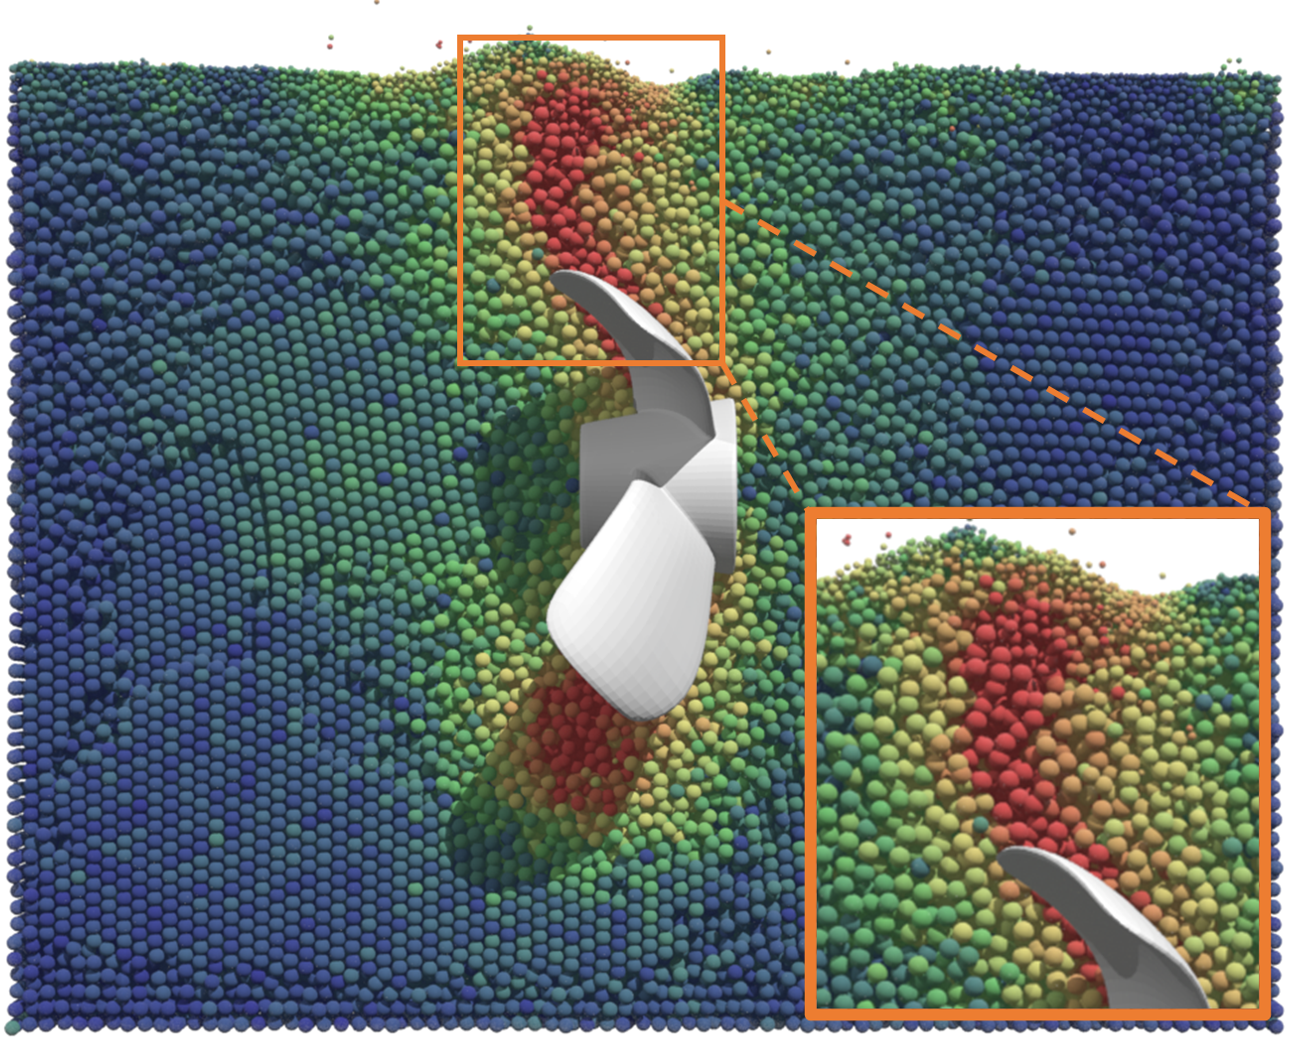
\includegraphics[width=0.31\textwidth]{figure/prop/surface.png}
\label{fig:prop_surface}
}
\vspace{-0.7\baselineskip}
\caption{
A cross-section of the propeller spinning experiment where colour denotes velocity. Adaptive methods use $r_{base} = 0.1$, $\alpha = 32$, $\tau^{max}_{propeller} = 0$. In the zoomed-in areas, our method (b) generates a more detailed vortex compared to (c), closer to the high-resolution result (a).
% Propeller spinning experiment where a propeller rotates in the fluid. A cross-section of the fluid is displayed. Particle colour denotes velocity. Compared to the surface-based method (c), our method (b) generates a vortex (the zoomed-in area) with finer details, which is also more similar to the high-resolution simulation (a).
}
\label{fig:prop}

\end{figure}

\begin{figure*}
    \centering
    \subfigure[Our method without wake flow preservation ($\tau_{box}^{max} = 0$).]{
    
    \begin{overpic}[width=0.155\textwidth]{figure/box/box_schem_bound2.png}
    \put (19,17) {\footnotesize refine}
    \put (60,12) {\footnotesize fluid}
    \put (22,29.5) {\footnotesize box}
    \end{overpic}
    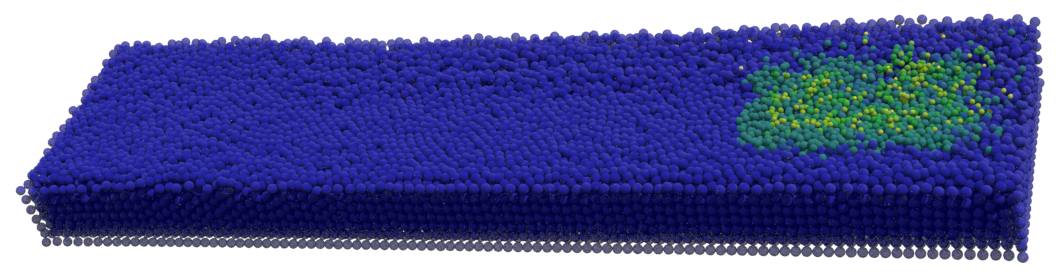
\includegraphics[width=0.27\textwidth]{figure/box/bound1.png}
    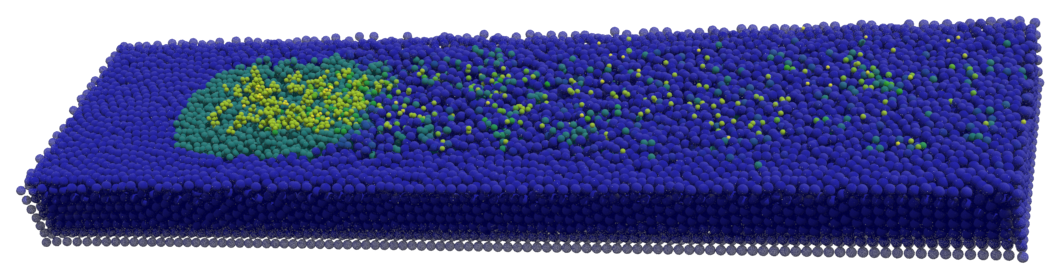
\includegraphics[width=0.27\textwidth]{figure/box/bound4.png}
    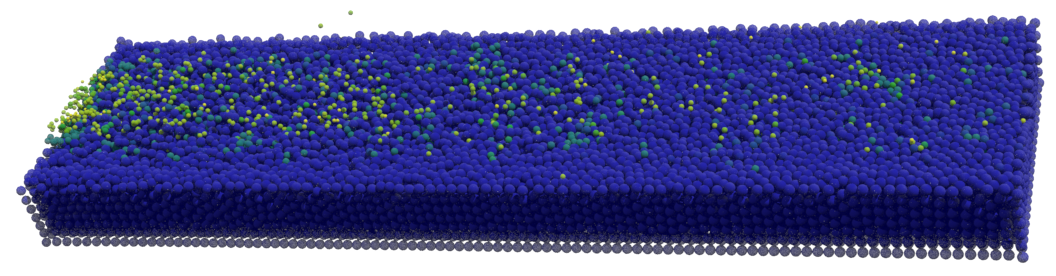
\includegraphics[width=0.27\textwidth]{figure/box/bound5.png}
    \label{fig:box_bound}
    }
    \subfigure[Our method with wake flow preservation ($\tau_{box}^{max} = 1$).]{
    
    \begin{overpic}[width=0.155\textwidth]{figure/box/box_schem_mark2.png}
    \put (19,17) {\footnotesize refine}
    \put (40,8.5) {\footnotesize fluid}
    \put (22,29.5) {\footnotesize box}
    \put (50,17) {\footnotesize wake flow}
    \end{overpic}
    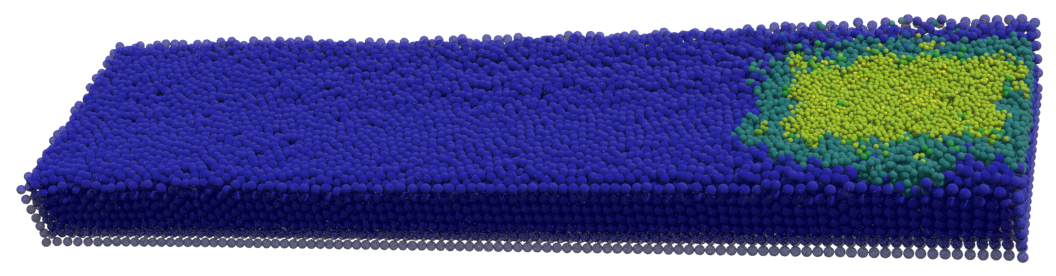
\includegraphics[width=0.27\textwidth]{figure/box/mark1.png}
    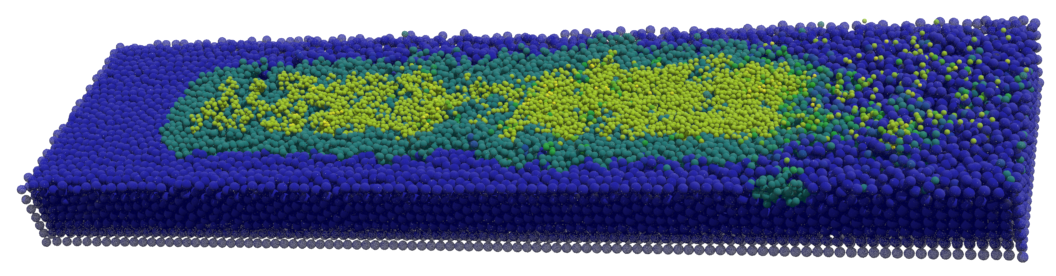
\includegraphics[width=0.27\textwidth]{figure/box/mark4.png}
    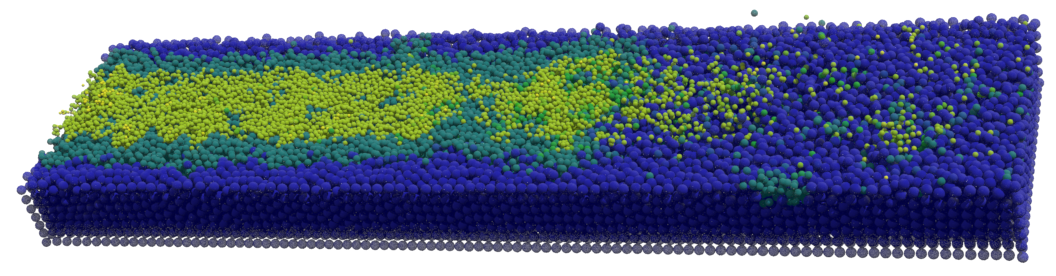
\includegraphics[width=0.27\textwidth]{figure/box/mark5.png}
    \label{fig:box_mark}
    }
    \vspace{-0.7\baselineskip}
    \caption{Moving box experiment. In this experiment, a box-shaped boundary object moves close to the fluid surface but not touching the fluid, causing particle refinement near it but not disturbing the fluid. The leftmost column shows the experimental setup; the other columns show the result. Color denotes particle size. Our method uses $r_{base} = 0.2$ and $\alpha = 32$. The distance between the box and the fluid surface is $0.1$.}
    
\end{figure*}

\begin{figure*}
    \centering
    \subfigure[Boat-sailing experiment.]{
    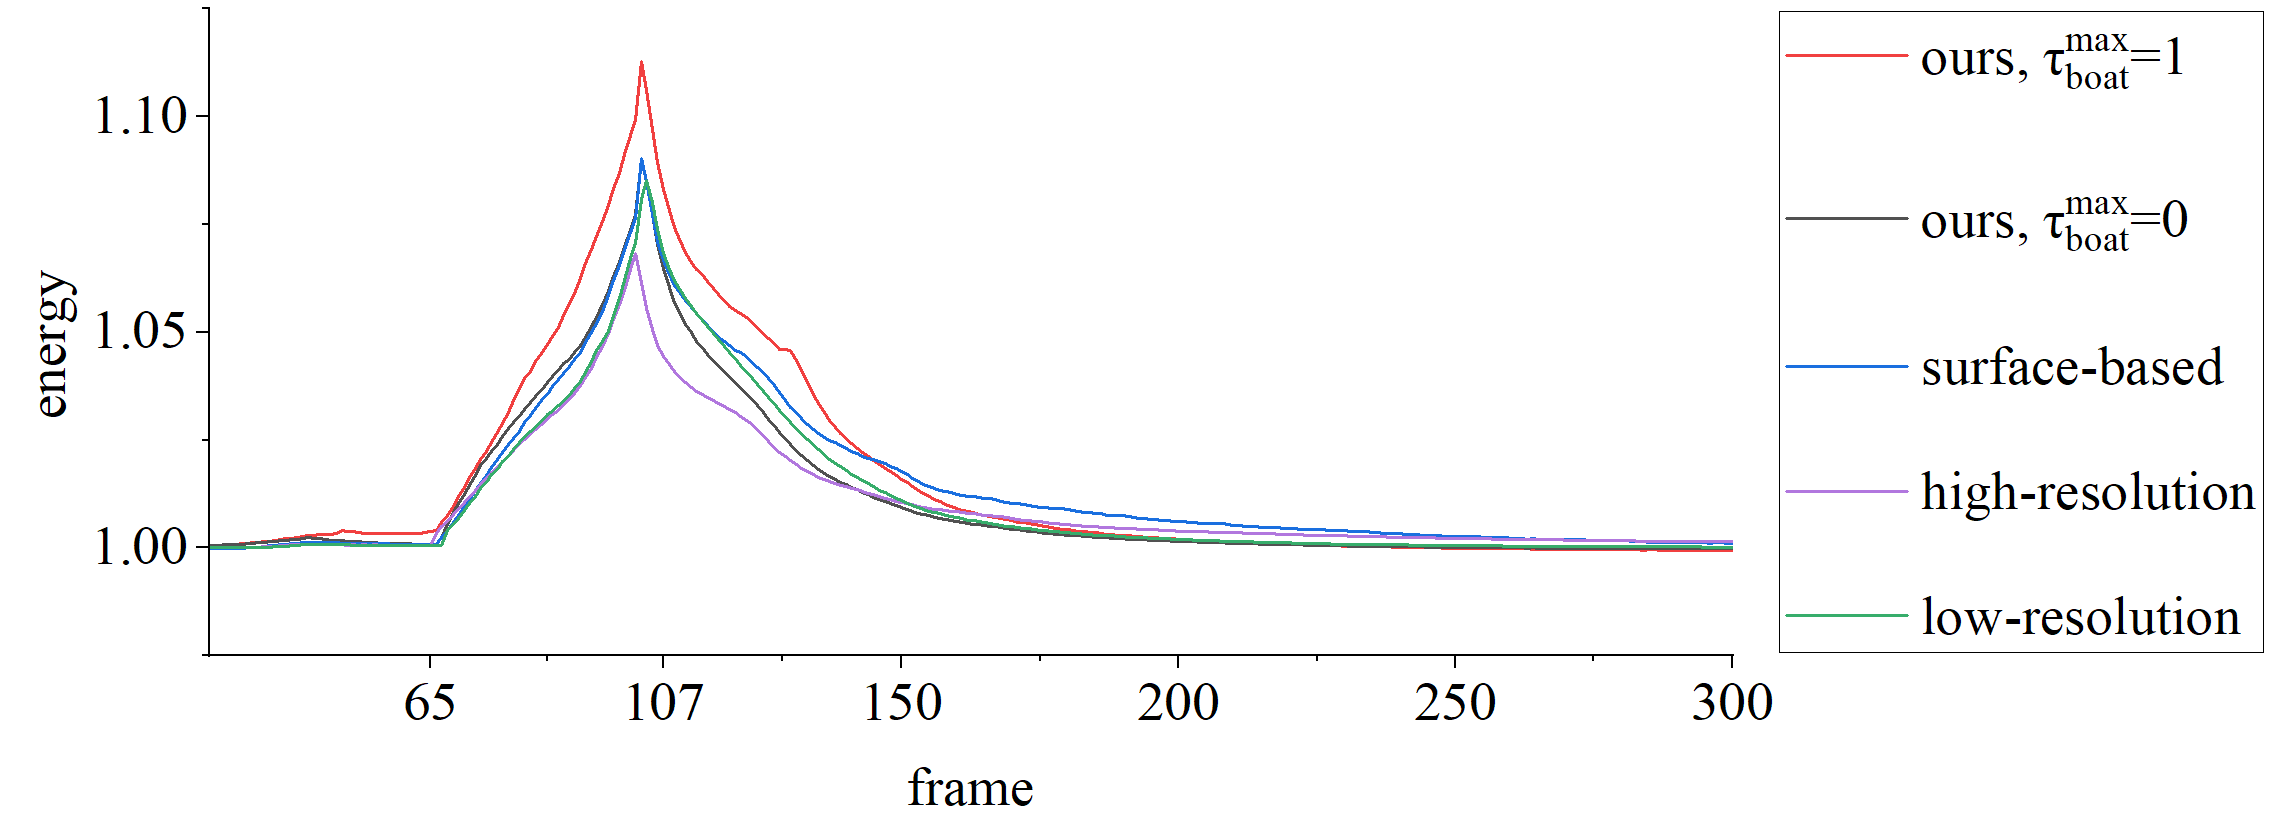
\includegraphics[width=0.635\textwidth]{figure/data/ship_energy.png}
    \label{fig:ship_energy}
    }
    \subfigure[Moving box experiment.]{
    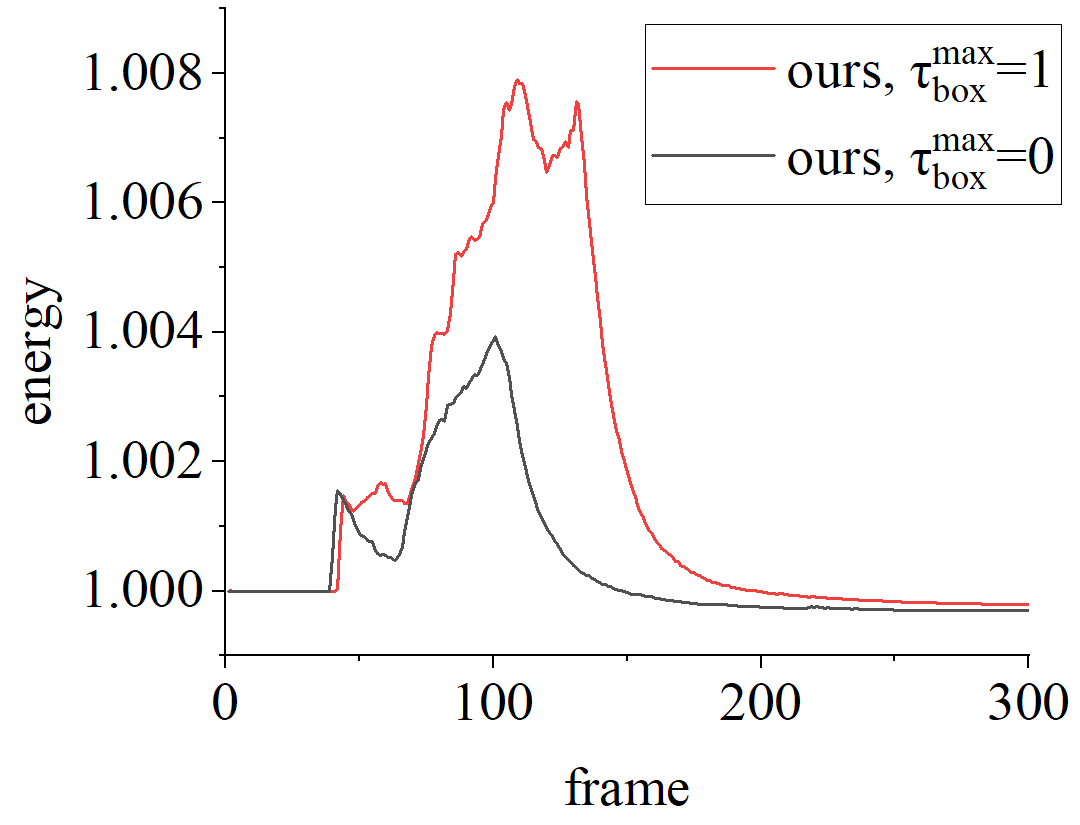
\includegraphics[width=0.3\textwidth]{figure/data/energy_box.png}
    \label{fig:energy_box}
    }
    \vspace{-0.7\baselineskip}
    \caption{Sum of total kinetic and dynamic energy in boat-sailing and moving box experiment, expressed in ratio of current energy to energy in the first frame. One frame equals $1/24\mathrm{s}$.}
    
\end{figure*}

\section{Conclusion and Discussion}

\section{Limitations}

\paragraph{visual performance}
In the surface-based only SPH adaptive mechanism, the sizes of the particles are always transformed smoothly in space according to a continuous and stable signed distance field. However, our boundary-based adaptive method may encounter the difficulties of particle merging. The divided small particles, as a part of the waves stirred up by the solid boundary, may not have the neighbour particles of similar size to be merged when falling back to the fluid surface.
 
We make a solid boundary fly over the fluid surface without substantive contact to demonstrate this issue. Only the sizes of the fluid particle will be affected by the signed distance field from the solid object. As shown in Fig.~\ref{}, we carried out this experiment separately with and without the wake flow preservation mechanism. The sizes of the particles are colour-coded as smaller particles with brighter appearances. Here we can see that our wake flow preservation mechanism delays the merging process effectively.

However, we can also observe that when the solid object leaves the fluid surface, some small particles are left unmerged on the surface. This is because our method only allows the merging procedure to happen between particles of similar sizes. When small particles begin to merge, there will be $s$ particles too far away from one another to be fused. On the other hand, the surface-based adaptive mechanism naturally guarantees fluid particles near each other obtain similar sizes as it only depends on particles' distances to the fluid surface.

\subsection{Summary}

We propose a new boundary refinement mechanism for adaptive SPH to refine particles near the coupling boundary and retain resolution for the flow generated by solid objects. 
%
Experiments show that, compared to surface-based only refinement mechanism, our method can improve the computation efficiency significantly for enhancing fluid details when simulating fluid-solid coupling scenarios. 
%
Further, the proposed method can also produce more accurate visual results for underwater coupling scenarios such as propeller spinning.
%
Therefore, our method can be widely applied to most fluid simulation scenarios to improve the efficiency and visual quality since many fluid simulations focus on the interaction between fluid and solid. 
%
A limitation of our method is that when a solid particle leaves the refined region due to splashing etc., it would lack merge partners and remain in the unrefined region, causing a small redundancy in particles. We aim to deal with this limitation in further research. In the future we will develop new mechanism to address this issue.


% \begin{figure}
% \centering
% \includegraphics[width=6cm]{figure.jpg}
% \caption{
% Diagrams aid a readers perception of the paper, to correctly convey information.}
% \label{fig:ex}
% \end{figure}

\section*{Acknowledgement}
This research was funded by: Horizon 2020-Marie Skłodowska-Curie Action-Individual Fellowships (No.895941), National Key Research and Development Program of China (No.2020YFB0704501), National Natural Science Foundation of China (No.61873299), Key Research and Development Project of Hainan Province (No.ZDYF2020031).

\nocite{*}% Show all bib entries - both cited and uncited; comment this line to view only cited bib entries;
\bibliography{example}

\section*{Author Biography}

\begin{biography}{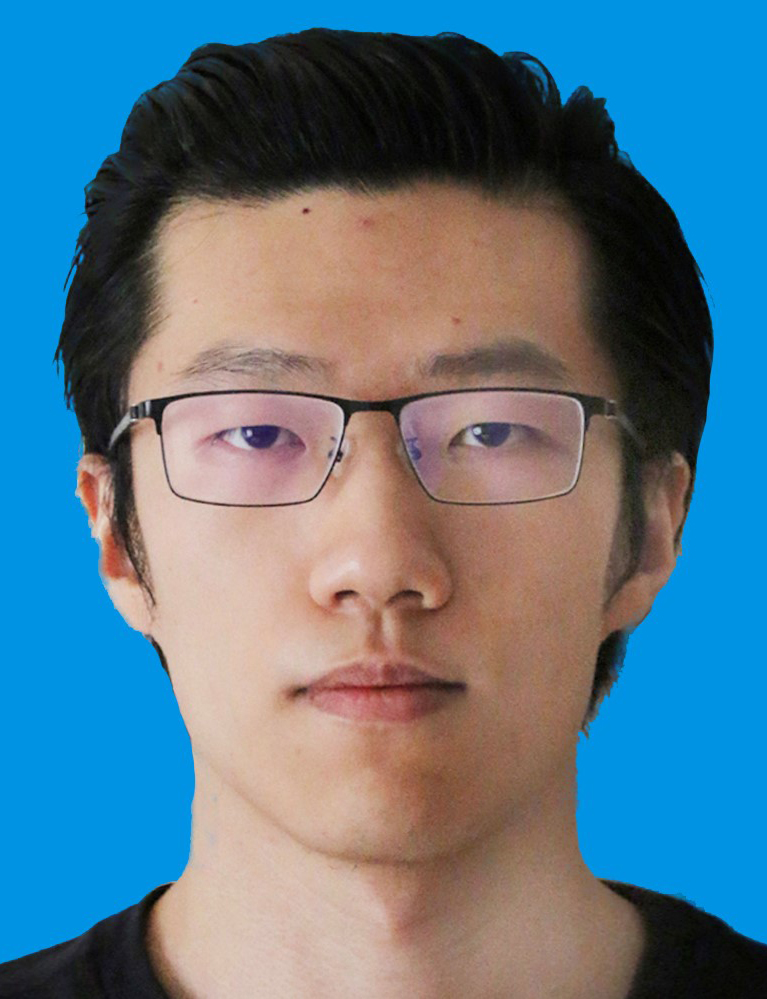
\includegraphics[width=66pt,height=86pt]{VANCOUVER/figure/photos/YanruiXu.jpg}}{\textbf{Yanrui Xu} is a Ph.D. student in Computer Science and Technology at University of Science and Technology Beijing. He received a Master's degree in University of Science and Technology Beijing, in 2020. His research field is computer graphics, especially physically-based fluid simulation.}
\end{biography}

\vspace{7ex}

\begin{biography}{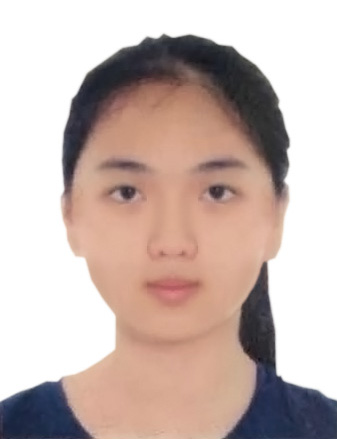
\includegraphics[width=66pt,height=86pt]{VANCOUVER/figure/photos/ChongmingSong.JPG}}{\textbf{Chongming Song} is a postgraduate student in Computer Science and Technology at University of Science and Technology Beijing. She received an undergraduate Diploma in University of Science and Technology Beijing, in 2021. Her research field is computer graphics, especially physically-based fluid simulation.}
\end{biography}

\vspace{7ex}

\begin{biography}{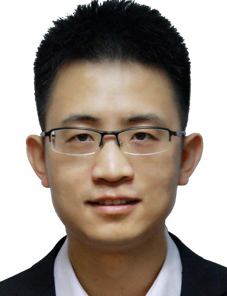
\includegraphics[width=66pt,height=86pt]{VANCOUVER/figure/photos/XiaokunWang.jpg}}{\textbf{Xiaokun Wang} is an associate professor in School of Computer and Communication Engineering, University of Science and Technology Beijing, China. He received a Ph.D. degree in Computer Science and Technology from University of Science and Technology Beijing, in 2017. His research interests include computer graphics, virtual reality and human-computer interaction.}
\end{biography}

\vspace{4.15ex}

\begin{biography}{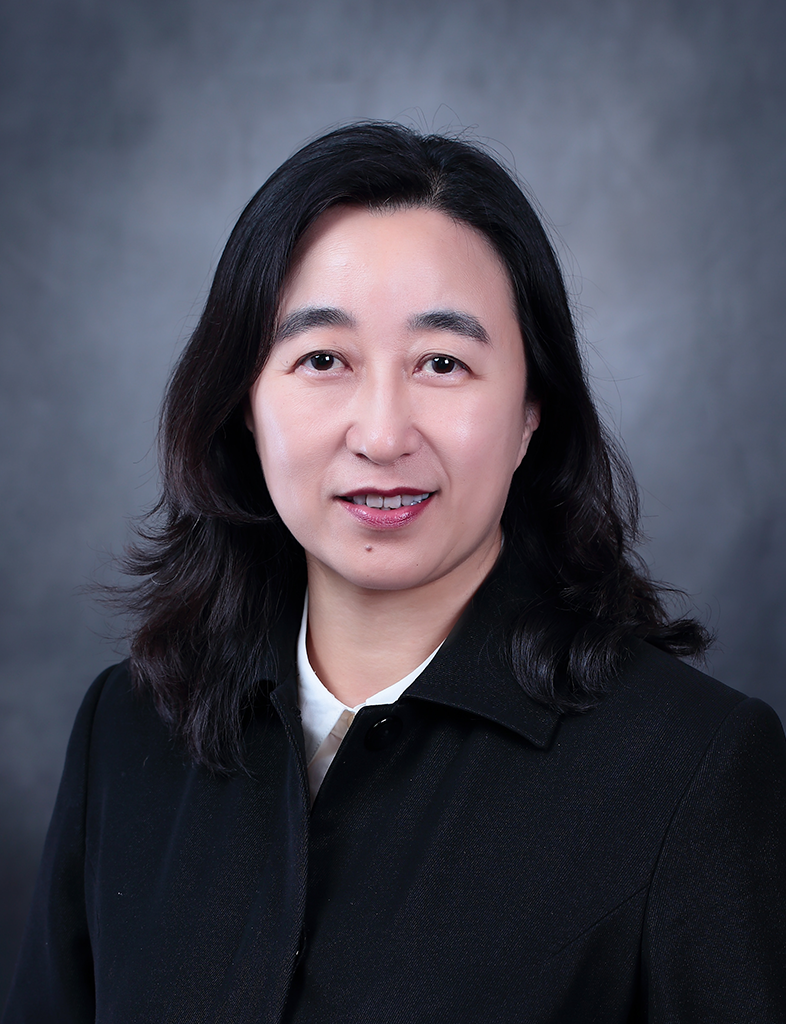
\includegraphics[width=66pt,height=86pt]{VANCOUVER/figure/photos/XiaojuanBan.png}}{\textbf{Xiaojuan Ban} is a professor in Artificial Intelligence and leader of the Computer Animation Group at University of Science and Technology Beijing, China. She received her master's degree in computer application and Ph.D. degree in control theory and control engineering from the University of Science and Technology Beijing. Her research interests include computer graphics, artificial intelligence, human-computer interaction, big data analysis and 3D visualization.}
\end{biography}

\vspace{1.3ex}

\begin{biography}{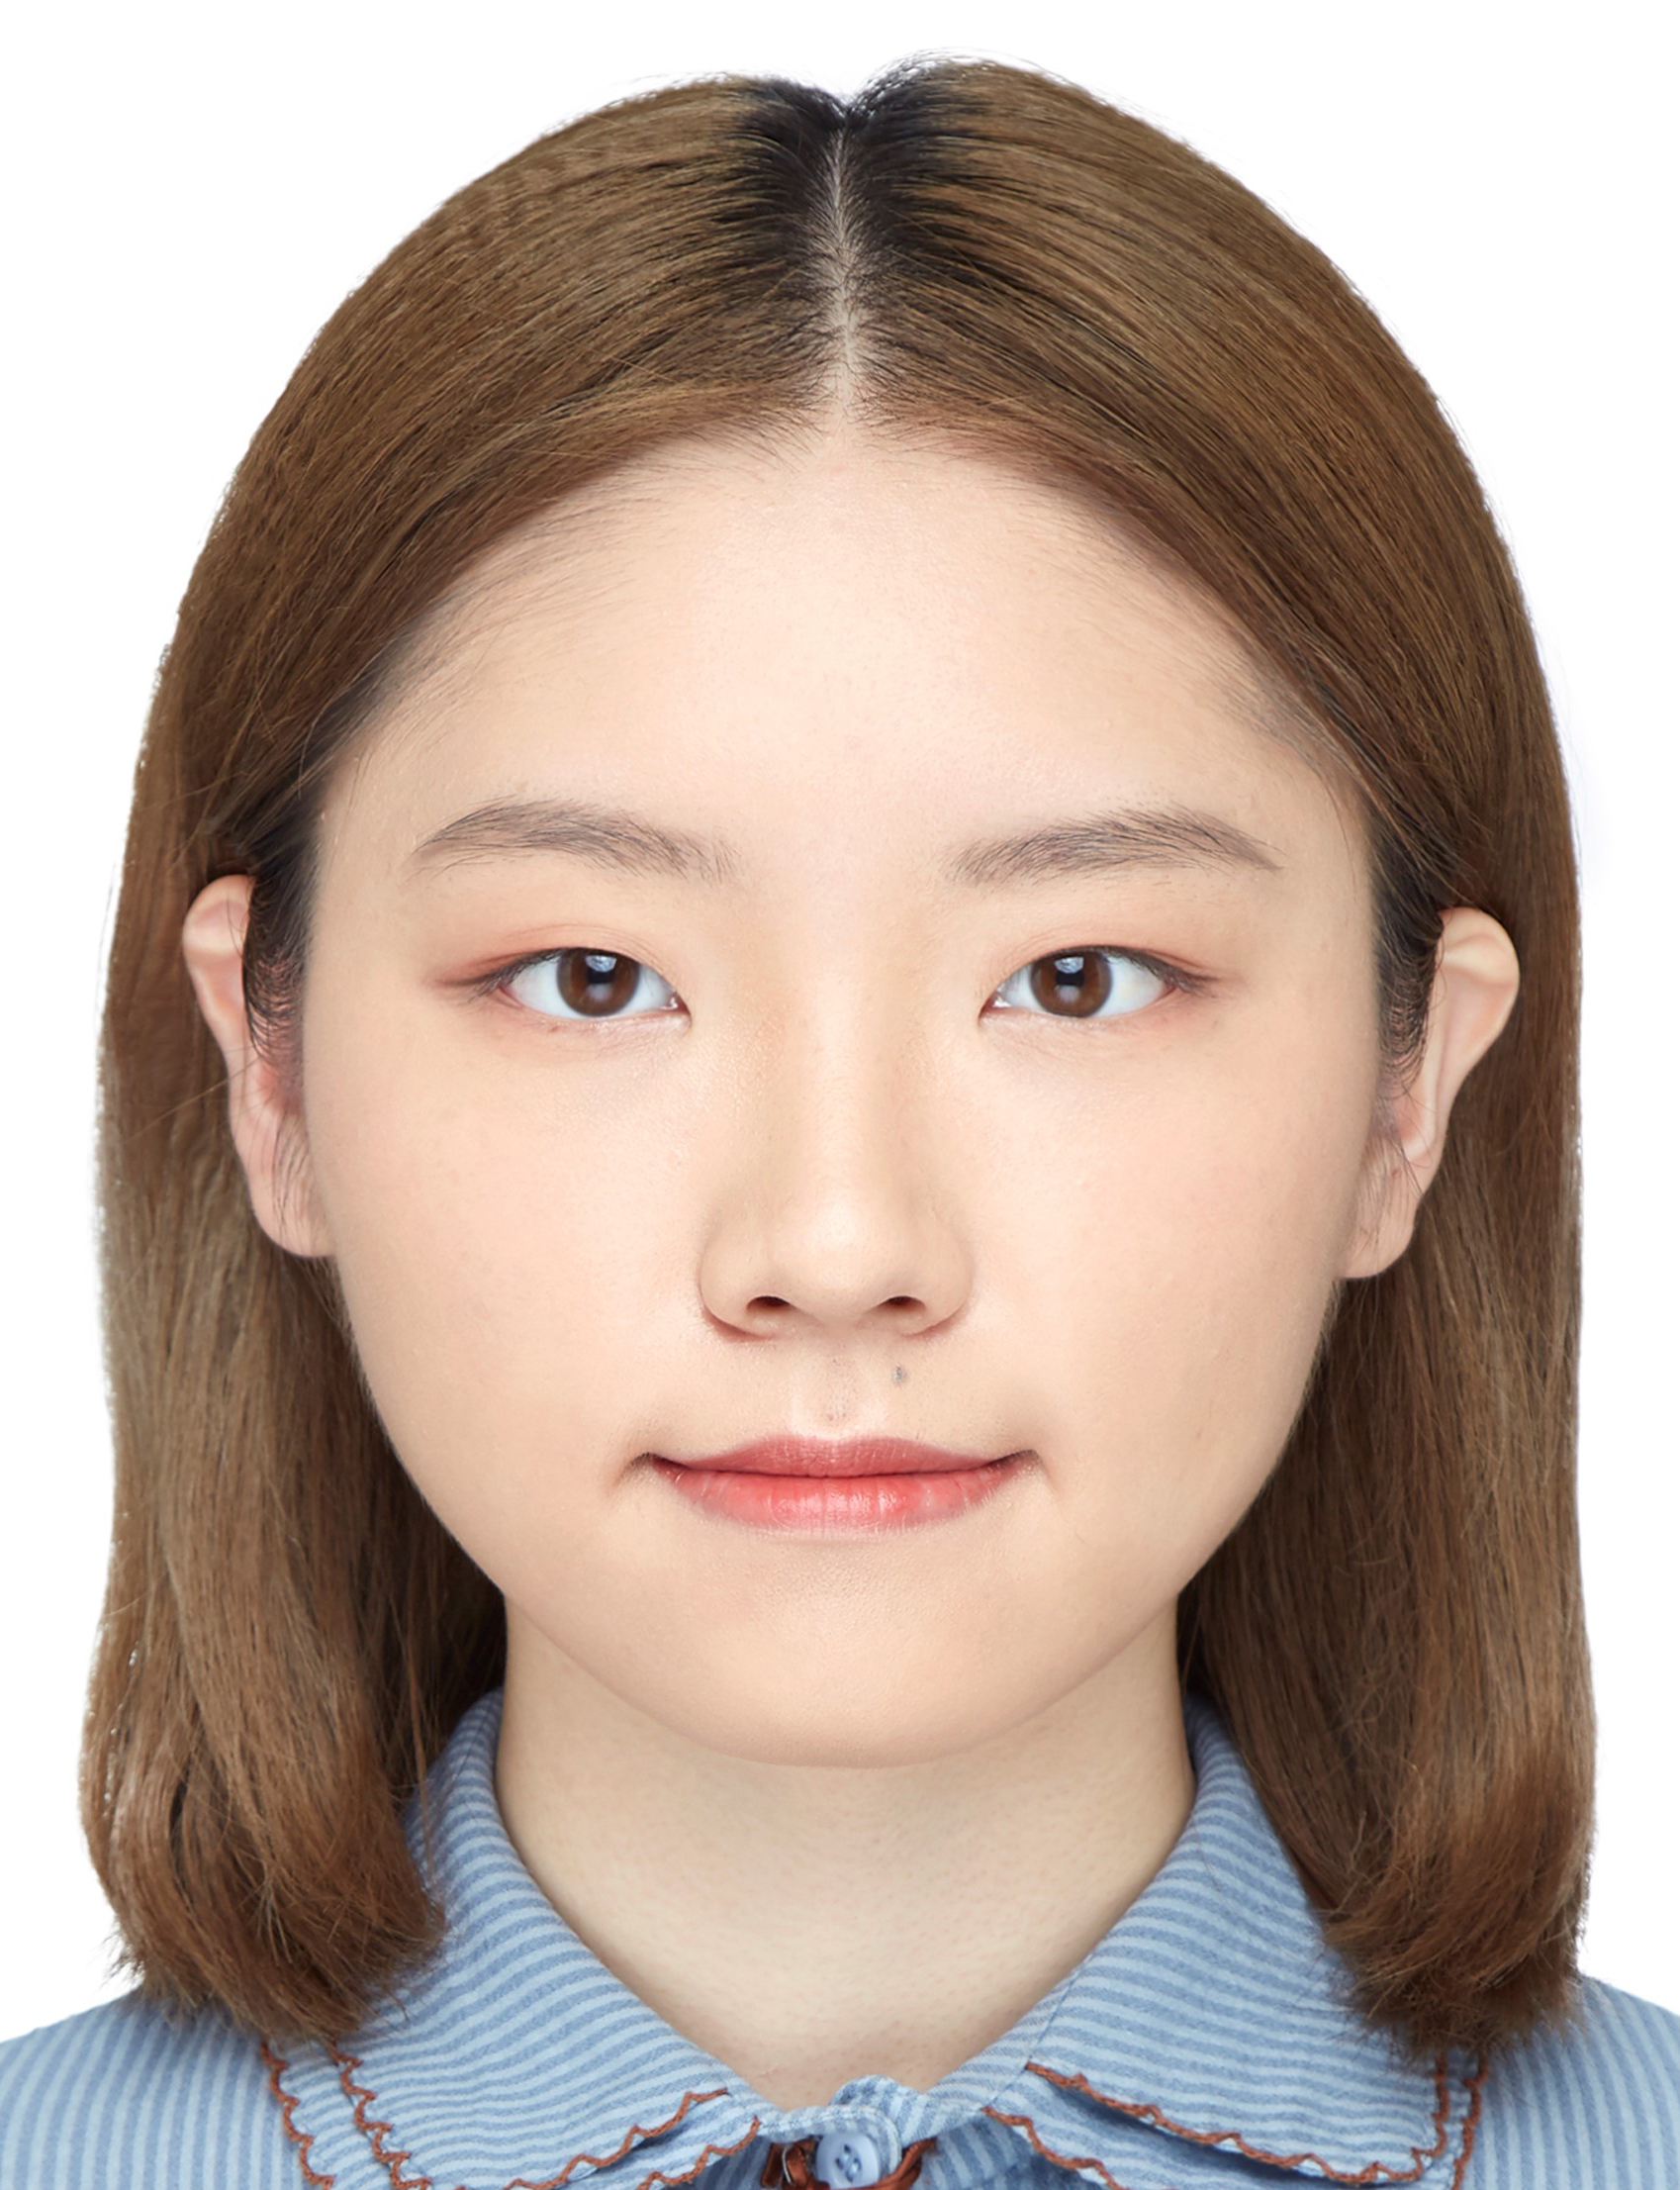
\includegraphics[width=66pt,height=86pt]{VANCOUVER/figure/photos/JiaminWang.jpg}}{\textbf{Jiamin Wang} is a postgraduate student in Computer Science and Technology at University of Science and Technology Beijing. She received an undergraduate Diploma in University of Science and Technology Beijing, in 2021. Her research field is computer graphics, especially physically-based fluid simulation.}
\end{biography}

\vspace{7ex}

\begin{biography}{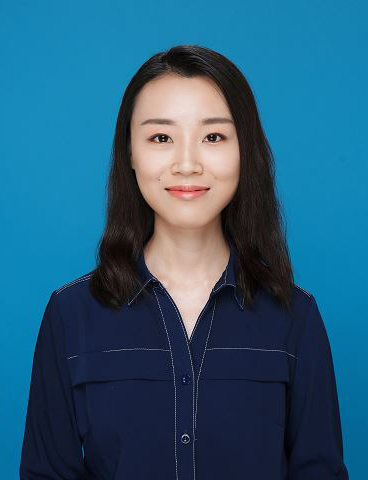
\includegraphics[width=66pt,height=86pt]{VANCOUVER/figure/photos/YalanZhang.jpg}}{\textbf{Yalan Zhang} received her Ph.D. degree in Computer Science and Technology from University of Science and Technology Beijing, China, in 2020. Currently, she is a lecturer at University of Science and Technology Beijing. Her research interests include computer graphics, 3-D visualization and computer vision.}
\end{biography}

\vspace{7ex}

\begin{biography}{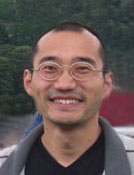
\includegraphics[width=66pt,height=86pt]{VANCOUVER/figure/photos/JianChang.jpg}}{\textbf{Jian Chang} is a professor in  computer animation at Bournemouth University, United Kindom. He received his Ph.D. degree in Computer Graphics from Bournemouth University, in 2007. His research interests include physics based modelling (deformation \& fluid), motion synthesis, virtual reality (surgery simulation), and novel HCI (eye tracking, gesture control and haptic).}
\end{biography}

\vspace{5ex}

\end{document}
